% coding: UTF-8
%photonics.tex
% Fundamental of Photonics

\documentclass{article}
%页眉
\usepackage{titleps,kantlipsum}
\newpagestyle{mypage}{
  \headrule 
  \sethead{\MakeUppercase{\thesubsection\quad \subsectiontitle}}{}{\thepage}
}
\settitlemarks{section,subsection,subsubsection}
\pagestyle{mypage}

%公式编号
\usepackage{mathtools}
\newtagform{mydefault}[\thesubsection-]{(}{)}
\usetagform{mydefault}
\makeatletter
\@addtoreset{equation}{subsection}
\makeatother

%插图
\usepackage{graphicx}
\usepackage{subfig}
\usepackage{float}

%颜色和color rectangle
\usepackage[dvipsnames]{xcolor}
\definecolor{ksc}{rgb}{0.24,0.36,0.65}
\definecolor{KSC}{named}{ksc}
\newcommand\crule[3][black]{\textcolor{#1}{\rule{#2}{#3}}}

%页面大小
\usepackage{geometry}
\geometry{a4paper,centering,scale=0.8}

%标题和日期
\title{\textcolor{ksc}{\textbf{\rightline{C H A P T E R}\\ \rightline{\Huge{11}}}}}
\date{}

%参考文献
\bibliographystyle{plain}

%目录
\renewcommand{\contentsname}{\textcolor{ksc}{STATISTICAL OPTICS}}
\renewcommand\thesection{\arabic{section}}
\renewcommand\thesubsection{\thesection.\arabic{subsection}}
\renewcommand\thesubsubsection{\Alph{subsubsection}.}
\renewcommand{\abstractname}{\null}
\setcounter{section}{11}

%图片和表格编号
\numberwithin{figure}{subsection}
\numberwithin{table}{subsection}
\renewcommand{\thefigure}{\thesubsection-\arabic{figure}}
\renewcommand{\thetable}{\thesubsection-\arabic{table}}

%微分算子优化和度定义
\usepackage{amsmath}
\DeclareMathOperator\dif{d\!}
\newcommand\degree{^\circ}

%行距
\usepackage{setspace}

%数学黑板粗体 P
\usepackage{amssymb}

%小黑色方块
\DeclareFontFamily{U}{MnSymbolC}{}
\DeclareFontShape{U}{MnSymbolC}{m}{n}{
  <-5.5> MnSymbolC5
  <5.5-6.5> MnSymbolC6
  <6.5-7.5> MnSymbolC7
  <7.5-8.5> MnSymbolC8
  <8.5-9.5> MnSymbolC9
  <9.5-11.5> MnSymbolC10
  <11.5-> MnSymbolCb12
}{}
\DeclareRobustCommand{\sqcdot}{%
  \mathbin{\text{\usefont{U}{MnSymbolC}{m}{n}\symbol{"69}}}%
}

%段落除首行缩进
\usepackage[notquote]{hanging}

\begin{document}
\nocite{*}
\maketitle
\noindent{\crule{\textwidth}{0.5cm}}
\tableofcontents

%摘要
\begin{abstract}
\begin{figure*}[h]
\centering
\subfloat[Max Born (1882-1970)]{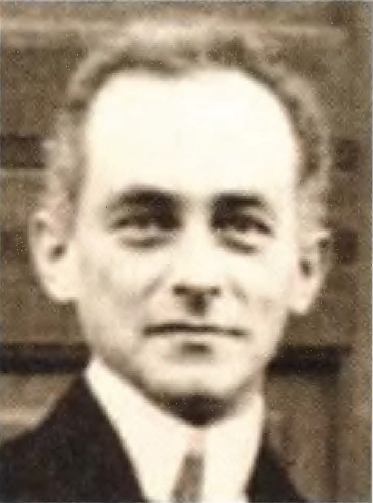
\includegraphics[width=0.2\textwidth]{maxborn.PNG}}
\hspace{.25in}
\subfloat[Emil Wolf (born 1922)]{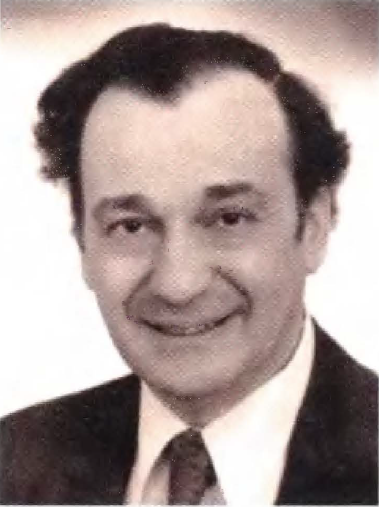
\includegraphics[width=0.2\textwidth]{emilwolf.PNG}}
\end{figure*}
The book Principle of Optics, first published in 1959 by Max Born and Emil Wolf, drew attetion 
to the importance of coherence in optics. Emil Wolf is responsible for many advances in the theory
of optical coherence.
\end{abstract}

\newpage\textbf{Statistical optics} is the study of properties of random light. Randomness in light
arises because of unpredictable fluctuations of the light source or of the medium 
through which light propagtes. Natural light, eg., light radiated by a hot object, is
random because it is a superstition of emissions from a very large number of atoms
radiating independently and at different frequencies and phases. Randomness in light
may also be a result of scattering from rough surfaces, diffused glass, or turbulent 
fluids, which impart random variations to optical wavefront. The study of the
random fluctuation of light is also known as the \textbf{theory of optical coherence}.
\par In the preceding chapters it was assumed that light is deterministic or  ``coherent.'' An
example of   coherent light is the monochromatic wave $ u(r,t) = Re \{ U(r) \exp(j\omega t) \}$,
for which the complex amplitude $ U(r) $ is a deterministic complex function, e.g., 
$ U(r) = Aexp(-jkr)/r $ in the case of  a spherical wave [Figure.11.0-1(a)].
The dependence of the wave function on time and position is perfectly periodic and 
predictable. On the other hand, for random light, the dependence of the wavefunction 
on time and position [Figure.11.0-1(b)] is not totally predicatable and cannot generally be 
described without resorting to statistical methods.  
\begin{figure}[H]
\centering
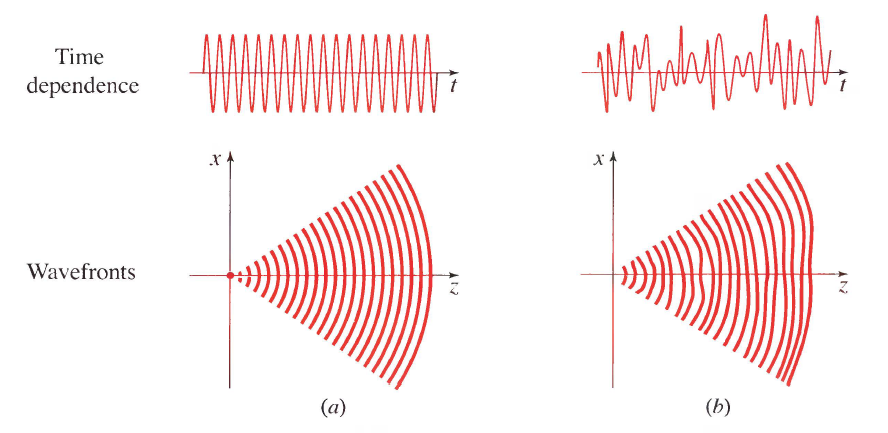
\includegraphics[width=0.9\textwidth]{11_0_1.PNG}
\caption{Time dependence and wavefronts of (a) a monochromatic spherical wave, which is an example of coherent light;
(b)random light.}
\label{fig: 11_0_1}
\end{figure}
\par How can we extract from the fluctuations of a random optical wave some meaningful
measures that characterize it and distinguish it from other random waves? Examine, for
instance, the three random optical waves whose wavefunctions at some position 
vary with time as in Fig.11.0-2. It is apparent that wave(b) is more ``intense'' than wave(a)
and that the envelope of wave(c) fluctuates ``faster'' than the envelopes of the other two waves.
\begin{figure}[ht]
\centering
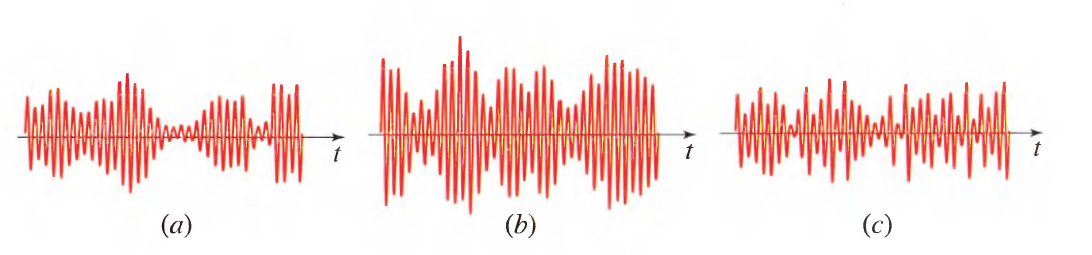
\includegraphics[width=0.9\textwidth]{11_0_2.PNG}
\caption{Time dependence of the wavefunctions of three random waves.}
\label{fig: 11_0_2}
\end{figure}
\par To translate these casual qualitative observations into quantitative measures, we use the concept of statistical averaging to define a number of nonrandom measures. Becasue the random function $ u(r,t) $
satisfies cetain laws(the wave equation and boundary conditions) its statistical averages must also satify certain laws. The theory of optical coherence deals with the definitions of these statistical averages, with the laws that govern them, and with measures by which light is classified as \textbf{coherent, incoherent, \textnormal{or, in general,} paritially coherent}.
\bigbreak\noindent\textcolor{ksc}{\textbf{\textsl{This Chapter}}}
\par This chapter is an introduction to the theory of partial coherence. Familiarity with the
theory of random fields (random functions of many variables — space and time) is
necessary for a full understanding of the theory of optical coherence. However, the
ideas presented in this chapter are limited in scope, so that knowledge of the concept
of statistical averaging is sufficient.
In Sec. 11.1 we define two statistical averages used to describe random light: the optical
intensity and the mutual coherence function. Temporal and spatial coherence are
delineated, and the connection between temporal coherence and monochromaticity is
established. The examples of partially coherent light provided in Sec. 11.1 demonstrate
that spatially coherent light need not be temporally coherent, and that monochromatic
light need not be spatially coherent. One of the basic manifestations of the coherence
of light is its ability to produce visible interference fringes. Sec. 11.2 is devoted to the
laws of interference of random light. The transmission of partially coherent light in
free space and through different optical systems, including image-formation systems,
is the subject of Sec. 11.3. A brief introduction to the theory of polarization of random
light(partial polarization) is provided in Sec. 11.4.

\bigbreak\begingroup
\color{ksc}
\subsection{STATISTICAL PROPERTY OF RANDOM LIGHT}
\endgroup
An arbitrary optical wave is described by a wavefunction $ u(r,t) = Re\{U(r,t)\} $, where $ U(r,t) $
is the complex wavefunction. For example, $ U(r,t) $ may take the form $ U(r)\exp(j\omega t)$
for monochromatic light, or it may be a sum of many similar functions of different $\nu$ for polychromatic light(see Sec. 2.6A  for a discussion of the complex wavefunction). For random 
light, both functions, $ u(r,t) $ and $ U(r,t) $ are random and are characterized by a number of statistical
averages introduced in this section.

\bigbreak\begingroup
\color{ksc}
\subsubsection{Optical Intensity}
\endgroup
The intensity $ I(r,t )$ of  coherent (deterministic) light is the absolute square of the complex wavefunction $ U(r,t) $,
\begin{equation}
I(r,t) = \lvert U(r,t) \rvert ^2 .
\end{equation}
(see Sec. 2.2A and Sec. 2.6A). For monochromatic deterministic light the intensity is independent of time, but for pulsed 
light it is time varying.
\par For random light, $ U(r,t) $ is a random function of time and postion. The intensity  $ \lvert U(r,t) \rvert ^2 $ is therefore also random.The \textbf{average intensity} is the defined as 
\begin{equation}
I(r,t) = \langle \lvert U(r,t) \rvert ^2 \rangle .
\end{equation}
where the symbol $ \langle \cdot \rangle $ now denotes an ensemble average over many realizations of the random function. This means that the wave
is produced repeatedly under the same conditions, with each trial yielding a different wavefunction, and the average intensity at each time and position is determined. When there is no ambiguity we shall simply call $ I(r,t) $ the intensity of light (with the word \textsl{average} implied).
The quality $ \lvert U(r,t) \rvert ^2 $ is called the \textbf{random} or \textbf{instantaneous intensity}. For deterministic light, the averaging operation is unnecessary since all trials produce the same wavefunction, so that (11.1-2) is equivalent to (11.1-1).
\par The average intensity may be time independent or may be a function of time, as illustrated in Figs. 11.1-1(a) and (b), respectively. The former case applies when the optical wave is statistically \textbf{stationary}; that is, its statistical averages are invariant to time. The instantaneous intensity fluctuates randomly with time, but its average is constant.
We will denote it, in this case, by $ I(r) $. Stationary does not necessarily mean constancy. It means constancy of the average properties. An example of stationary random light is that from an ordinary incandescent lamp heated by a constant electric current. The average intensity $ I(r) $ is a function of distance from the lamp, but it does not vary with time. However, the random intensity $ \lvert U(r,t) \rvert ^2 $ fluctuates with both position and time, as illustrated in Fig.11.1-1(a).
\begin{figure}[ht]
\centering
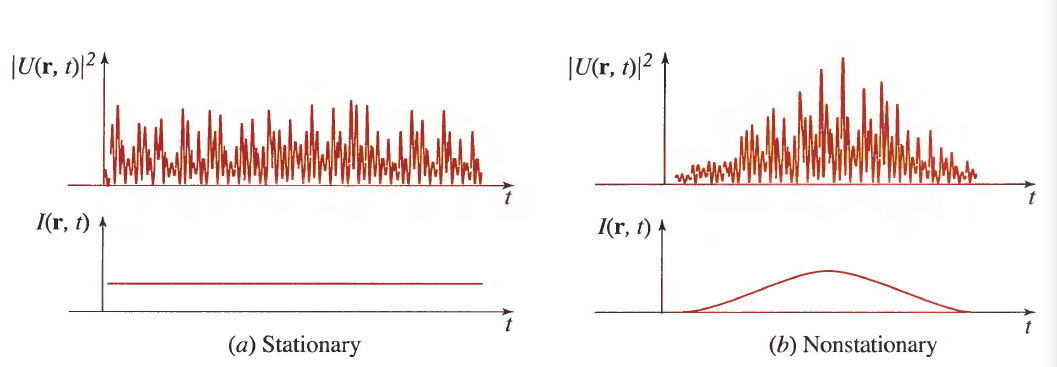
\includegraphics[width=0.9\textwidth]{11_1_1.PNG}
\caption{(a) A statistically stationary wave has an average intensity that does not vary with time. (b) A statistically nonstationary wave has a time-varying intensity. These plots represent, e.g., the intensity of light  from an incandescent lamp driven by a constant eletric current in (a) and a pulse of electric current in (b).}
\label{fig: 11_1_1}
\end{figure}
\par When the light is stationary, the statistical averaging operation in (11.1-2)  can usually be determined by time averaging over a long time(instead of averaging over many realizations of the wave), whereupon
\begin{equation}
I(r) = \lim_{T\to\infty}\frac{1}{2T} \int_{-T}^T \lvert U(r,t) \rvert ^2 \dif t
\end{equation}

\bigbreak\begingroup
\color{ksc}
\subsubsection{Temporal Coherence and Spectrum}
\endgroup
Consider the fluctuations of \textsl{stationary} light at a fixed position $ r $ as a function of time. The stationary random function $ U(r,t) $ has a constant intensity $ I(r) = \langle \lvert U(r,t) \rvert \rangle ^2 $. For brevity, we drop the $ r $ dependence(since $ r $ is fixed), so that $ U(r,t) = U(t) $ and $ I(r)=I $.
\par The random fluctuation of $ U(t) $ are characterized by a time scale representing ``memory'' of the random function. Fluctuations at points seperated by a time interval longer than the memory time are independent, so that the process ``forgets'' itself. The function appears to be smooth within its memory time, but ``rough'' and ``erratic''  when examined over longer time scales(see Fig. 11.0-2). A quantitative measure of this temporal behavior is established by defining a statistical \textsl{average} known as the autocorrelation function. This function describes the extent to which the wave function fluctuates in unison at two instants of time saparated by a given time delay, so that it establishes the time scale  of the process that underlies the generation of the wavefunction.
\bigbreak\noindent\textcolor{ksc}{\textbf{\textsl{Temporal Coherence Function}}}\\
The autocorrelation function of a stationary complex random function $ U(t)  $ is the average of the product of $ U^\ast (t) $ and $ U(t+\tau) $ as a function of the time delay $ \tau $ 
\begin{equation}
G(\tau) = \langle U^\ast (t)U(t+\tau) \rangle
\end{equation}
or
\begin{equation}
G(\tau) = \lim_{T\to\infty}\frac{1}{2T} \int_{-T}^T U^\ast (t)U(t+\tau) \dif t
\end{equation}
(see Sec. A.1 in Appendix A).
\par To understand the significance of the definition in (11.1-4), consider the case in which the average value of the complex wavefunction $\langle U(t) \rangle = 0 $. This is applicable when the phase of phasor $U(t)$ is equally likely to have any value between 0 and $ 2\pi $, as illustrated in Fig. 11.1-2. The phase of the product $ U^\ast (t)U(t+\tau) $ is the angle beween phasors $ U(t) $ and $ U(t+\tau) $. If $ U(t) $ and $ U(t+\tau) $ are uncorrelated, the angle between their phasors varies randomly between 0 and $ 2\pi $. The phasor $ U^\ast (t)U(t+\tau) $ then has a totally uncertain angle, so that it is equally likely to take any direction, making its average, the autocorrelation function $ G(\tau) $, vanish. On the other hand if, for a given $ \tau$, $ U(t) $ and $ U(t+\tau) $ are correlated, their phasors will maintain some relationship. Their fluctuations are then linked together so that the product phasor $ U^\ast (t)U(t+\tau) $ has a preferred direction and its average $ G(\tau) $ will not vanish.
\begin{figure}[ht]
\centering
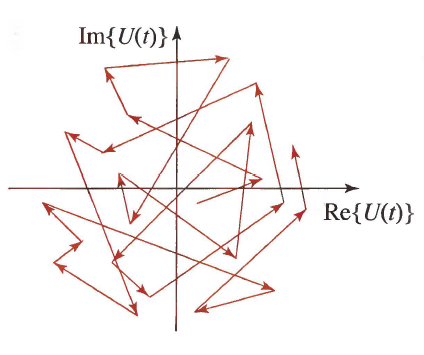
\includegraphics[width=0.4\textwidth]{11_1_2.PNG}
\caption{Variation of phasor $ U(t) $ with time when its argument is uniformly distributed between 0 and $ 2\pi $. The average values of its real and imaginary parts are zero, so that $ \langle U(t) \rangle = 0 $.}
\label{fig: 11_1_2}
\end{figure}
\par In the language of optical coherence theory, the autocorrelation function $ G(\tau) $ is known as the \textbf{temporal coherence function}. It is easy to show that $ G(\tau) $ is a function with Hermitian symmetry, $ G(-\tau) = G^\ast (\tau) $, and that the intensity $ I $, defined by (11.1-2), is equal to $ G(\tau) $ when $ \tau =0 $,
\begin{equation}
I = G(0).
\end{equation}
\bigbreak\noindent\textcolor{ksc}{\textbf{\textsl{Degree of Temporal Coherence}}}\\
The temporal coherence function $ G(\tau) $ carries information about both the intensity $ I = G(0) $ and degree of correlation (coherence) of stationary light. A measure of coherence that is insenstive to the intensity is provided by the normalized autocorrelation function,
\begin{equation}
g(\tau) = \frac{G(\tau)}{G(0)} = \frac{\langle U^\ast (t)U(t+\tau) \rangle}{\langle U^\ast (t)U(t) \rangle},
\end{equation}
which is called the \textbf{complex degree of temporal coherence}. It is absolute value cannot exceed unity,
\begin{equation}
0\leq \lvert g(\tau) \rvert \leq 1
\end{equation}
\par The value of $ \lvert g(\tau) \rvert $ is a measurement of the degree of correlation between $ U(t) $ and $ U(t+\tau) $. When the light is deterministic and monochromatic, i.e., $ U(t) =A \exp(j\omega_0 t) $, where A is constant, (11.1-7) gives
\begin{equation}
g(\tau) = \exp(j\omega_0 \tau),
\end{equation} 
so that $ g(\tau) = 1$ for all $ \tau $. The variables $ U(t) $ and $ U(t+\tau) $ are then completely correlated for all time delays $ \tau $. Usually, $ \lvert g(\tau) \rvert $ drops from its largest value $ g(0) = 1 $ as $ \tau $ increases and the fluctuations become uncorrelated for a sufficiently large $ \tau $.
\bigbreak\noindent\textcolor{ksc}{\textbf{\textsl{Coherence Time}}}\\
If $\lvert g(\tau) \rvert $ decreases monotonically with time delay, the value $ \tau_c $ at which it drops to a prescribed value ($ \frac{1}{2} $ or $ \frac{1}{e} $, for example) serves as a measure of the memory time of the fluctuations known as the \textbf{coherence time} (see Fig. 11.1-3).
\begin{figure}[H]
\centering
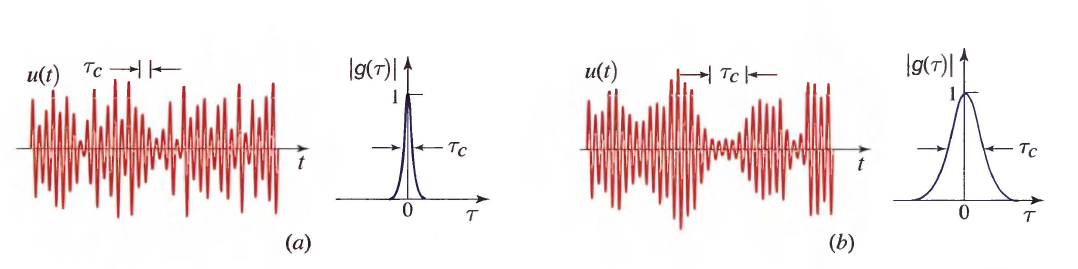
\includegraphics[width=0.9\textwidth]{11_1_3.PNG}
\caption{Illustrative examples of the wavefunction, the magnitude of the complex degree of
temporal coherence $\lvert g(\tau) \rvert $, and the coherence time $ \tau_c $ for an optical field with (a) short coherence time and (b) long coherence time. The amplitude and phase of the wavefunction vary randomly with time
constants approximately equal to the coherence time. In both cases the coherence time $ \tau_c $ is greater
than the duration of an optical cycle. Within the coherence time, the wave is rather predictable and can
be approximated as a sinusoid. However, given the amplitude and phase of the wave at a particular
time, one cannot predict the amplitude and phase at times beyond the coherence time.}
\label{fig: 11_1_3}
\end{figure}
\par For $\tau < \tau_c $ the fluctuations are ``strongly'' correlated whereas for $ \tau > \tau_c $ they are ``weekly'' correlated. In general, $ \tau_c $ is the width of the function  $\lvert g(\tau) \rvert $. Although the definition of the width of a function is rather arbitray (see Sec. A.2 of Appendix A), the power-equivalent width
\begin{equation}
\tau_c = \int_{-\infty}^{+\infty} \lvert g(\tau) \rvert ^2 \dif \tau
\end{equation}
is commonly used as the definition of coherence time [see (A.2-8) and note that $ g(0) = 1$]. The coherence time of monochromatic light is infinite since $\lvert g(\tau) \rvert = 1$ everywhere.
\bigbreak\noindent{\crule[ksc]{\textwidth}{0.2cm}}
\textbf{EXERCISE 11.1-1} \\
\textbf{Coherence Time.} Verify that the following expressions for the complex degree of temporal coherence are consistent with the definition of $ \tau_c $ given in (11.1-10):
\begin{equation}
g(\tau) = 
\begin{cases}
\exp(-\frac{\lvert \tau \rvert}{\tau_c}) & (exponential) \\
\exp(-\frac{\pi \tau^2}{2\tau_c^2}) & (Gaussian)
\end{cases}
\end{equation}
By what factor does $ \lvert g(\tau) \rvert $ drop as $ \tau $ increases from 0 to $ \tau_c $ in each case? \\
\noindent{\crule[ksc]{\textwidth}{0.2cm}}
\par Light for which the coherence time $ \tau_c $ is much longer than the differences of the time delays encountered in the optical system of interest is effectively completely coherent. Thus, light is effectively coherent if the distance $c\tau_c$ is much greater than all optical path-length differences encountered. The distance
\begin{equation}
l_c = c\tau_c
\end{equation}
is known as the \textbf{coherence length}.
\bigbreak\noindent\textcolor{ksc}{\textbf{\textsl{Power Spectral Density}}}\\
To determine the \textsl{average} spectrum of random light, we carry out a Fourier decomposition of the random function $ U(t) $. The amplitude of the component with frequency $ \nu $ is the Fourier transform (see Appendix A)
\begin{equation}
V(\nu) = \int_{-\infty}^{+\infty} U(t) \exp(-j2 \pi \nu t) \dif t .
\end{equation}
The average energy per unit area of those components with frequencies in the interval between $ \nu $ and $ \nu +\dif \nu $ is $ \langle \lvert V(\nu) \rvert ^2 \rangle \dif \nu $, so that  $ \langle \lvert V(\nu) \rvert ^2 \rangle $ represents the energy spectral density of the light (energy per unit area). Note that the complex wave function $ U(t) $ has been defined so that $ V(\nu) = 0 $ for negative $ \nu $ (see Sec. 2.6A).
\par Since a truly stationary function $ U(t) $ is eternal and carries infinte energy, we consider instead the \textsl{power} spectral density. We first determine the energy spectral density of the function $ U(t) $ observed over a window of time width T by finding the truncated Fourier transform
\begin{equation}
V_T (\nu) = \int_{-T/2}^{+T/2} U(t) \exp(-j2 \pi \nu t) \dif t
\end{equation}
and then determine the energy spectral density   $ \langle \lvert V_T (\nu) \rvert ^2 \rangle $. The power spectral density is the energy per unit time $ (1/T) \langle \lvert V_T (\nu) \rvert ^2 \rangle $.  We can now extend the time window to infinity by taking the limit $ T \to \infty $. The result
\begin{equation}
S(\nu) = \lim_{T \to \infty} \frac{1}{T} \langle \lvert V_T (\nu) \rvert ^2 \rangle ,
\end{equation}
is called the \textbf{power spectral density}. It is nonzero only for positive frequencies. Because $ U(t) $ was defined such that $ \lvert U(t) \rvert^2 $ represents power per unit area, or intensity ($ W/cm^2 $), $ S(\nu) \dif \nu $ represents the average power per unit area carried by frequencies between $ \nu $ and $ \nu + \dif \nu $, so that $ S(\nu) $ actually represents the \textbf{intensity spectral density} ($ W/cm^2 -Hz $). It is often referred to simply as the \textbf{spectral density} or the \textbf{spectrum}. The total average intensity is the integral
\begin{equation}
I = \int_0^\infty S(\nu) \dif \nu .
\end{equation}
\par The autocorrelation function $ G(\tau) $, defined by (11.1-4), and the spectral density $ S(\nu) $ defined by (11.1-15) can be shown to form a Fourier transform pair (see Prob. 11.1-5),
\begin{equation}
S(\nu) = \int_{-\infty}^{+\infty} G(\tau) \exp(-j2 \pi \nu \tau) \dif \tau .
\end{equation}
This relation is known as the \textbf{Wiener-Khinchin theorem}.\\
\par An optical wave representing a color image, such as that illustrated in Fig. 11.1-4, has a spectrum that varies with position $ r $; each spectral profile shown corresponds to a perceived color.
\begin{figure}[ht]
\centering
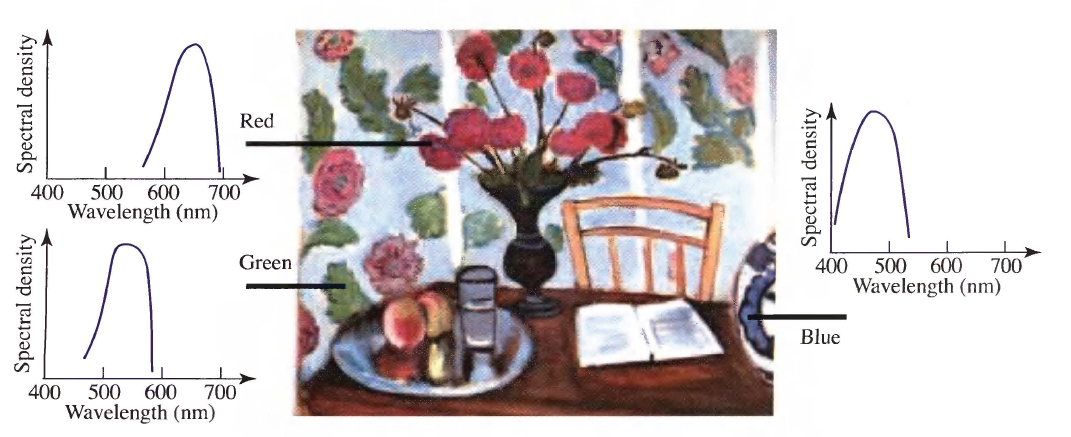
\includegraphics[width=0.9\textwidth]{11_1_4.PNG}
\caption{Variation of the spectral density as a function of wavelength at three postion in a color image (Dahlias,Henri Matisse).}
\label{fig: 11_1_4}
\end{figure}
\bigbreak\noindent\textcolor{ksc}{\textbf{\textsl{Spectral Width}}}\\
The spectrum of light is often confined to a narrow band centered about a central frequency $ \nu_0 $. The \textbf{spectral width}, or \textbf{linewidth}, of light is the width $ \Delta \nu $ of the spectral density $ S(\nu) $. Because of the Fourier-transform relation between $ S(\nu) $ and $ G(\tau) $, their widths are inversely related. A light source of broad spectrum has a short coherent time, whereas a light source with narrow linewidth has a long coherence time, as illustrated in Fig. 11.1-5. In the limiting case of monochromatic light, $ G(\tau) = I \exp(j\omega_0 \tau) $, so that the corresponding intensity spectral density $ S(\nu) = I \delta (\nu - \nu_0) $ contains only a single frequency component, $ \nu_0 $. Thus, $ \tau_c = \infty $ and $ \Delta \nu = 0$. The coherence time of a light source can be increased by using an optical filter to reduce its spectral width. The resultant gain of coherence comes at the expense of losing light energy.
\begin{figure}[H]
\centering
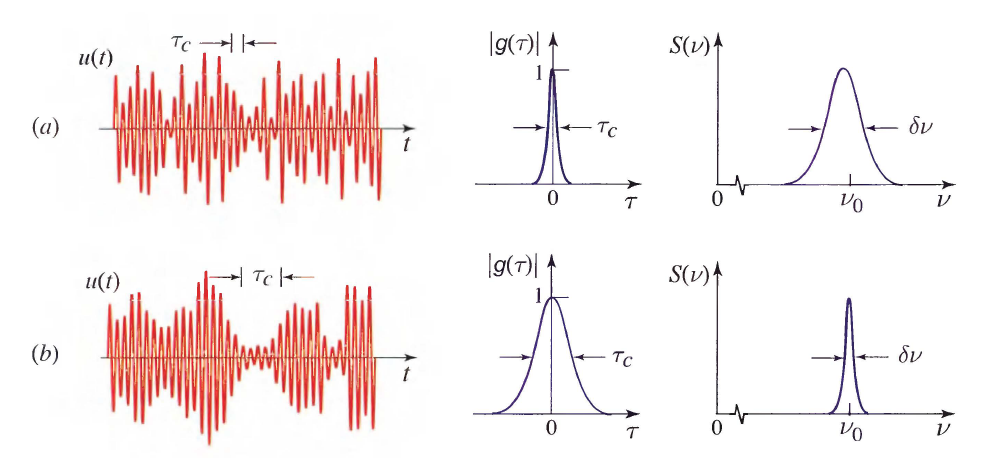
\includegraphics[width=0.9\textwidth]{11_1_5.PNG}
\caption{Two random waves, the magnitudes of their complex degree of temporal coherence, and their spectral densities.}
\label{fig: 11_1_5}
\end{figure}
\par There are several definitions for the spectral width. The most common is the full width of the function $ S(\nu) $ at half its maximum value (FWHM). The relation between the coherence time and the spectral width depends on the spectral profile, as indicated in Table 11.1-1 (see also Appendix A, Sec. A.2).\\
\begin{table}
\caption{Relation between spectral width and coherence time.}
\begin{center}
\begin{tabular}{lccc}
\hline
Spectral Density & Reactangular & Lorentzian & Gaussian \\
\hline
Spectral Width $ \delta \nu_{FWHM} $ & $ \frac{1}{\tau_c} $ & $ \frac{1}{\pi \tau_c} \approx \frac{0.32}{\tau_c} $ & $ \frac{\sqrt{2 ln2 / \pi}}{\tau_c} \approx \frac{0.66}{\tau_c} $ \\
\hline
\end{tabular}
\end{center}
\end{table}
\par Another convenient definition of the spectral width is
\begin{equation}
\Delta \nu_c = \frac{(\int_0^\infty S(\nu) \dif \nu)^2}{\int_0^\infty S^2(\nu) \dif \nu}.
\end{equation}
\par By this definition it can be shown that
\begin{equation}
\Delta \nu_c = \frac{1}{\tau_c},
\end{equation}
regardless of the spectral profile (see Exercise 11.1-2). If $ S(\nu) $ is a rectangular function extending over a frquency interval from $ \nu_0 - B/2 $ to $ \nu_0 + B/2 $, for example, then (11.1-18) yields $ \Delta \nu_c = B $. The two definitions of bandwidth, $ \Delta \nu_c $ and $ \Delta \nu_{FWHM} \equiv \Delta \nu $, differ by a factor that ranges from $1/\pi \approx 0.32 $ to 1 for the profiles listed in Table 11.1-1.
\bigbreak\noindent{\crule[ksc]{\textwidth}{0.2cm}}
\textbf{EXERCISE 11.1-2} \\
\textbf{Relation Between Spectral Width and Coherence Time.} Show that the coherence time $ \tau_c $ defined by (11.1-10) is related to the spectral width $ \Delta \nu_c $ defined in (11.1-18) by the simple inverse relation $ \tau_c = 1/ \Delta \nu_c $. Hint: Use the definition of $ \Delta \nu_c $ and  $ \tau_c $, the Fourier translation between $ S(\nu) $ and $ G(\tau) $, and Parseval's theorem [see (A.1-7) in Appendix A].\\
\noindent{\crule[ksc]{\textwidth}{0.2cm}}
\par Representative spectral bandwiths for different light sources, and their associated coherence times and coherence lengths $ l_c = c\tau_c$, are provided in Table 11.1-2.
\begin{table}[H]
\caption{Spectral widths of a number of light sources together with their coherence times and coherence lengths in free space.}
\begin{center}
\begin{tabular}{lccc}
\hline
Source & $ \Delta \nu_c (Hz) $ & $ \tau_c = 1/\Delta \nu_c $ & $ l_c = c\tau_c $ \\
\hline
Filtered sunlight ($ \lambda_0 = 0.4-0.8 \mu m $) & $ 3.74\times 10^14 $ & $ 2.67 fs $ & $ 800 nm $ \\
Light-emmiting diode ($ \lambda_0 = 1\mu m, \Delta \lambda_0 = 50 nm $) & $ 1.5\times 10^13 $ & $ 67 fs$ & $ 20 \mu m $ \\
Low-pressure sodium lamp & $ 5\times 10^11 $ & $ 2 ps $ & $ 600 \mu m $ \\
Mutimode He-Ne laser ($ \lambda_0 = 633 nm $) & $ 1.5 \times 10^9 $ & $ 0.67 ns $ & $ 20 cm $ \\
Single Mode He-Ne laser ($ \lambda_0 = 633 nm $) & $ 1\times 10^6 $ & $ 1 \mu s $ & $ 300 m $ \\
\hline
\end{tabular}
\end{center}
\end{table}
\noindent{\crule[ksc]{\textwidth}{0.1cm}}
\textbf{EXAMPLE 11.1-1. A Wave Comprising a Random Sequence of Wavepackets.} Light emitted from a incoherent source may be modeled as a sequence of wavepackets emitted at random times (Fig. 11.1-6). Each wavepacket has a random phase since it is emitted by a different atom.
\begin{figure}[H]
\centering
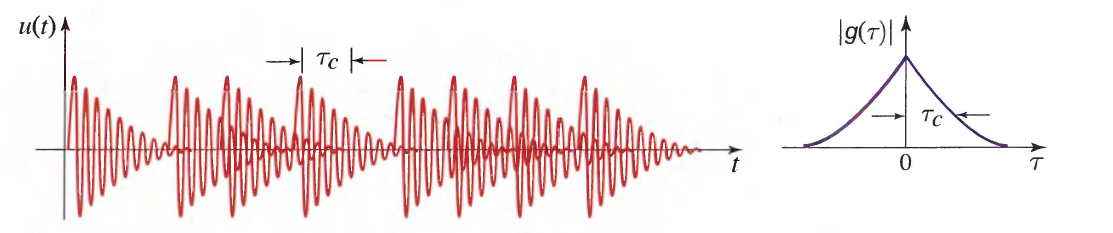
\includegraphics[width=0.9\textwidth]{11_1_6.PNG}
\caption{Light comprised of wavepackets emitted at random times has a coherence time equal to the duration of a wavepacket.}
\label{fig: 11_1_6}
\end{figure}
The wavepackets may be sinusoidal with an exponentially decaying envelope, for example, so that
a wavepacket emitted at $ t = 0 $ has a complex wavefunction (at a given position)
\begin{equation}
U_p(t) = 
\begin{cases}
A_p \exp(-\frac{t}{\tau_c}) \exp(j \omega_0 t), & t\geq 0 \\
0, & t < 0 .
\end{cases}
\end{equation}
The emission times are totally random, and the random independent phases of the different emissions are included in $ A_p $. The statistical properties of the total field may be determined by performing the necessary averaging operations using the rules of mathematical statistics. The result yields a complex degree of coherence given by $ g(\tau) = \exp(- \lvert \tau \rvert / \tau_c) \exp(j \omega_0 \tau) $ whose magnitude is a double-sided exponential function. The corresponding power spectral indensity is Lorentzian, $ S(\mu) = (\Delta \mu /2 \pi)/ [(\mu - \mu_0)^2 + (\Delta \mu /2)^2] $, where $ \Delta \mu = 1/ \pi \tau_c $ (see Table A.2-1 in Appendix A). The coherence time $ \tau_c $ in this case is exactly the width of a wavepacket. The statement that this light is correlated within the coherence time therefore means that it is correlated within the duration of an individual wavepacket.\\
\noindent{\crule[ksc]{\textwidth}{0.1cm}}

\bigbreak\begingroup
\color{ksc}
\subsubsection{Spatial Coherence}
\endgroup
\noindent\textcolor{ksc}{\textbf{\textsl{Mutual Coherence Function}}}\\
An important descriptor of the spatial and temporal fluctuations of the random function $ U(r,t) $ is the cross-correlation function of $ U(r_1,t) $ and $ U(r_2,t) $ at pairs of positions $ r1 $ and $ r2 $.
\begin{equation}
G(r_1, r_2, \tau) = \langle U^\ast (r_1, t) U(r_2, t + \tau) \rangle .
\end{equation}
This function of the time delay $\tau$ is known as the \textbf{mutual coherence function}. Its nomalized form,
\begin{equation}
g(r_1, r_2, \tau) = \frac{G(r_1, r_2, \tau)}{\sqrt{I(r_1) I(r_2)}},
\end{equation} 
is called the \textbf{complex degree of coherence}. When the two points coincide so that $ r_1 = r_2 = r $, (11.1-21) and (11.1-22) reproduce the temporal coherence function and the complex degree of temporal coherence defined in (11.1-4) and (11.1-7) at the position $ r $. Ultimately, when $ \tau = 0 $, the intensity $ I(r) = G(r, r, 0) $ at position $ r $.
\par The complex degree of coherence $ g(r_1, r_2, \tau) $ is the cross-correlation cofficient of the random variables $ U^\ast (r_1, t) $ and $ U(r_2, t + \tau) $ . Its absolute value is bounded between zero and unity,
\begin{equation}
0 \leq \lvert g(r_1, r_2, \tau) \rvert \leq 1 .
\end{equation}
It is therefore considered a measure of the degree of correlation between the fluctuation at $ r_1 $ and $ r_2 $ at a time $ \tau $ later.
\par When the two phasors $ U(r_1, t) $ and $ U(r_2, t) $ fluctuate independently and their phases are totally random (each havig equally probable between 0 and $ 2\pi $), $ g(r_1, r_2, \tau) = 0 $ since the average of the product $ U^\ast (r_1, t) U(r_2, t + \tau) $ vanishes. The light fluctuations at the two points are then uncorrelated. The other limit, $ g(r_1, r_2, \tau) = 1 $, applies when the light fluctuations at  $ r_1 $, and at $ r_2 $ a time $ \tau $ later, are fully correlated. Note that $ \lvert g(r_1, r_2, 0) $ is not necessarily unity; however, by definition$ g(r, r, 0) = 1 $.
\par The dependence of $ g(r_1, r_2, \tau) $ on time delay and on the positions characterizes the temporal and spatial coherence of light. Two examples of the dependence of  $ g(r_1, r_2, \tau) $ on distance $ \lvert r_1 - r_2 \rvert $ and the time delay $ \tau $ are illustrated in Fig. 11.1-7.
\begin{figure}[H]
\centering
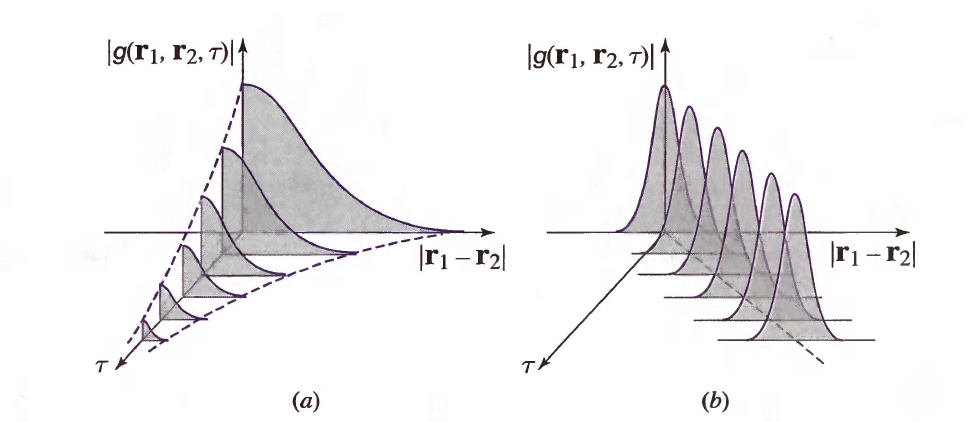
\includegraphics[width=0.9\textwidth]{11_1_7.PNG}
\caption{Two examples of $ g(r_1, r_2, \tau) $ as a function of the separation $ \lvert r_1 - r_2 \rvert $ and the time delay $ \tau $. In (a) the maximum correlation for a given $ \lvert r_1 - r_2 \rvert $ occurs at $ \tau = 0 $. In (b) the maximum correlation occurs at $ \lvert r_1 - r_2 \rvert = c \tau $. }
\label{fig: 11_1_7}
\end{figure}
\par The temporal and spatial fluctuations of  light are intimately related since light propagates in waves and the complex wavefunction $ U(r,t) $ must satisfy the wave equation. This imposes certain conditions on the mutual coherence function (see Exercise 11.1-3). To illustrate this point, consider, for example, a plane wave of random light traveling in the $ z $ direction in a homogeneous and nondispersive medium with velocity c. Fluctuations at the points $ r_1 = (0, 0, z_1) $ and $ r_2 = (0, 0, z_2) $ are completely correlated when the time delay is $ \tau = \tau_0 \equiv \lvert z_2 - z_1 \rvert /c $, so that $ \lvert g(r_1, r_2, \tau_0) \rvert = 1 $. As a function of $ \tau $, $ g(r_1, r_2, \tau) $ has a  peak at $ \tau = \tau_0 $, as illustrated in Fig. 11.1-7(b). This example will be discussed again in Sec. 11.1D.\\
\noindent{\crule[ksc]{\textwidth}{0.2cm}}
\textbf{EXERCISE 11.1-3} \\
\textbf{Differential Equations Governing the Mutual Coherence Function.} In free space, $ U(r,t) $ must satisfy the wave function, $ \nabla^2 U - (1/c^2  \partial^2 U / \partial t^2 = 0 $. Use the defintion (11.1-21) to show that the mutual coherence function $ G(r_1, r_2, \tau) $ satisfies the two partial differential equations
\begin{subequations}
\begin{align}
\nabla_1^2 G - \frac{1}{c^2} \frac{\partial^2 G}{\partial \tau^2}  &= 0\\
\nabla_2^2 G - \frac{1}{c^2} \frac{\partial^2 G}{\partial \tau^2 } &= 0,
\end{align}
\end{subequations} 
where $ \nabla_1^2 $ and $ \nabla_2^2 $ are the Laplacian operators with respect to $ r_1 $ and $ r_2 $, respectively.\\
\noindent{\crule[ksc]{\textwidth}{0.2cm}}
\bigbreak\noindent\textcolor{ksc}{\textbf{\textsl{Mutual intensity}}}\\
The spatial correlation of light may be assessed by examining the dependence of the mutual coherence function on position for a fixed time delay $ \tau $. In many situations the point $ \tau = 0 $ is the most appropriate, as in the example in Fig. 11.1-7(a). However, this need not always be the case, as in the example in Fig. 11.1-7(b). The mutual coherence function at $ \tau = 0 $,
\begin{equation}
G(r_1, r_2, 0) = \langle U_\ast (r_1, t) U(r_2, t) \rangle ,
\end{equation}
is known as the \textbf{mutual intensity} and is denoted by $ G(r_1, r_2) $ for simplicity. The diagonal values of the mutual intensity($ r_1 = r_2 = r $) provide the intensity $ I(r) = G(r,r) $.
\par When the optical path differences encoutered in an optical system are much shorter than the coherence length $ l_c = c\tau_c $, the light may be considered to effectively posses complete temporal coherence, so that the mutual coherence of function is a harmonic function of time:
\begin{equation}
G(r_1, r_2, \tau) = G(r_1, r_2) \exp(j\omega_0 \tau),
\end{equation}
where $ \nu_0 $ is the central frequency. In this case the light is said to be \textbf{quasi-monochromatic} and the mutual intensity $ G(r_1, r_2) $ decribes the spatial coherence completely.
\par The complex degree of coherence $ g(r_1, r_2, 0) $ is similarly denoted by $ g(r_1, r_2) $. Thus,
\begin{equation}
g(r_1, r_2) = \frac{G(r_1, r_2)}{\sqrt{I(r_1) I(r_2)}}
\end{equation}
is the normalized mutual intensity. The magnitude $ \lvert g(r_1, r_2) \rvert $ is bounded between zero and unity and is regarded as a measure of the degree of spatial coherence (when the time delay $ \tau $ is zero). If the complex wavefunction $ U(r, t) $ is deterministic, $ \lvert g(r_1, r_2) = 1 \rvert$ for all $ r_1 $ and $ r_2 $, so that the light is completely correlated everywhere.
\bigbreak\noindent\textcolor{ksc}{\textbf{\textsl{Coherence Area}}}\\
The spatial coherence of quasi-monochromatic light in a given plane in the vicinity of a given position $ r_2 $ is described by $ \lvert g(r_1, r_2) \rvert $ as a function of the distance $ \lvert r_1 - r_2 \rvert $. This function is unity when $ r_1 = r_2 $ and drops as $ \lvert r_1 - r_2 \rvert $ increases (but it need not be monotonic). The area scanned by the point $ r $ within which the function $ \lvert g(r_1, r_2) \rvert $ is greater than some prescribed value ($ \frac{1}{2} $ or $ \frac{1}{e} $, for example) is called the \textbf{coherence area}. It represents the spatial extent of $ \lvert g(r_1, r_2) \rvert $ as a function of $ r_1 $ for fixed $ r_2 $, as illustrated in Fig. 11.1-8. In the ideal limit of coherent light the coherence area is infinite.
\par The coherence area is an important parameter that characterizes random light. This parameter must be considered in relation to other pertinent dimensions of the optical system. For example, if the area of coherence is greater than the size of the aperture through which light is transmitted, so that $ \lvert g(r_1, r_2) \rvert \approx 1 $ at all points of interest, the light may be regarded as coherent, as if the coherence area where infinite. Similarly, if the coherence area is smaller than the resolution of the optical system, it can be regarded as infinitesimal, i.e., $ g(r_1, r_2) = 0 $ for practically all $ r_1 \neq r_2 $. In this limit the light is said to be \textbf{incoherent}.
\par Light radiated from an extended radiating hot surface has an area of coherence on the order of $ \lambda^2 $, where $ \lambda $ is the central wavelength, so that for most practical cases it may be regarded as incoherent. Thus, complete coherence and incoherence are only idealizations representing the two limits of partial coherence.
 \begin{figure}[H]
\centering
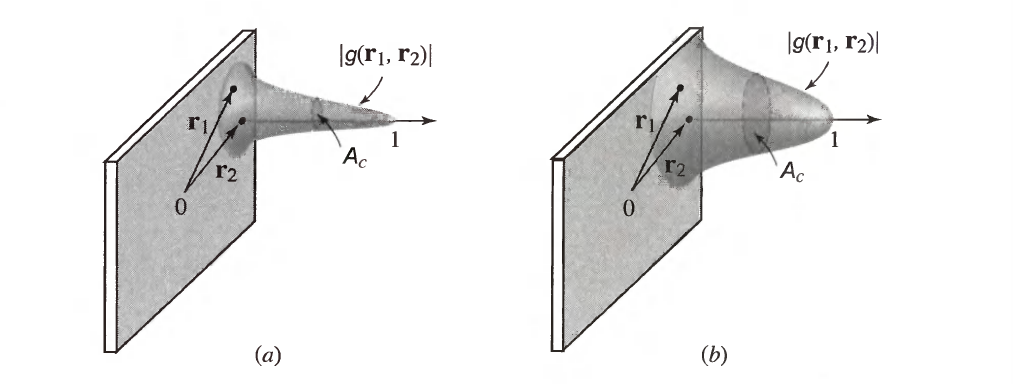
\includegraphics[width=0.9\textwidth]{11_1_8.PNG}
\caption{Two illustrative examples of the magnitude of the normalized mutual intensity as a function of $ r_1 $ in the vicinity of a fixed point $ r_2 $. The coherence area in (a) is samller than thar in (b).}
\label{fig: 11_1_8}
\end{figure}
\bigbreak\noindent\textcolor{ksc}{\textbf{\textsl{Cross-Spectral Density}}}\\
The mutual coherence function $ G(r_1, r_2, \tau) $ descibes the spatial correlation at each time delay $ \tau $. The time $ \tau = 0 $ is selected to define the mutual intensity $ G(r_1, r_2) = G(r_1, r_2, 0) $, which is suitable for decribing the spatial coherence of quasi-monochromatic light. A useful alternative is to describe coherence in the frequency domain by examining the spatial correlation at a fixed frequency. The \textbf{cross-spectral density} (or the cross-power spectrum) is defined as the Fourier transform of $ G(r_1, r_2, \tau) $ with respect to $ \tau $:
\begin{equation}
S(r_1, r_2, \nu) = \int_{-\infty}^{+\infty}G(r_1, r_2, \tau) \exp(-j2\pi \nu \tau) \dif \tau .
\end{equation}
When $ r_1 = r_2 = r $, the cross-spectral density becomes the power-spectral density $ S(\nu) $ at position $ r $, as defined in (11.1-17).
\par The normalized cross-spectral density is defined by
\begin{equation}
s(r_1, r_2, \nu) = \frac{S(r_1, r_2, \nu)}{\sqrt{S(r_1, r_1, \nu)S(r_2, r_2, \nu)}} ,
\end{equation}
and its magnitude camne shown to be bounded between zero and unity, so that it serves as a measure of the degree of spatial coherence at frequency $ \nu $. It represents the degree of correlation of the fluctuation components of frequency $ \nu $ at position $ r_1 $ and $ r_2 $.
\par In certain cases, the cross-spectral density factors into a product of one function of position and another of frequency, $ S(r_1, r_2, \nu) = G(r_1, r_2) s(\nu) $, so that the spatial and spectral properties are separable. The light is then said to be \textbf{cross-spectrally pure}. The mutual coherence function must then also factor into a product of a function of position and another of time, $ G(r_1, r_2, \tau) = G(r_1, r_2) g(\tau) $, where $ g(\tau) $ is the inverse Fourier transform of $ s(\nu) $. If the factorization parts are selected such that $ \int s(\nu) \dif \nu = 1 $, then $ G(r_1, r_2) = G(r_1, r_2, 0) $, so that $ G(r_1, r_2) $ is nothing but the mutual intensity. Cross-spectrally pure light has two important properties:
\par 1. At a single position $ r $, $ S(r, r, \nu) = G(r, r) s(\nu) = I(r) s(\nu) $. The spectrum has the same profiles at all positions. If the light represents a visible image, it would appear to have the same color everywhere but with varying brightness.
\par 2. The normalized cross-spectral density
\begin{equation}
s(r_1, r_2, \nu) = G(r_1, r_2) / \sqrt{G(r_1, r_1) G(r_2, r_2)} = g(r_1, r_2)
\end{equation}
is independent of frequency. In this case the normalized mutual intensity $ g(r_1, r_2) $ describes spatial coherence at all frequencies.

\bigbreak\begingroup
\color{ksc}
\subsubsection{Longitudinal Coherence}
\endgroup
In this section the concept of longitudinal coherence is introduced by taking examples of random waves with fixed wavefronts, such as planar and spherical waves.
\bigbreak\noindent\textcolor{ksc}{\textbf{\textsl{Partially Coherent Plane Wave}}}\\
Consider a plane wave
\begin{equation}
U(r, t) = a (t - \frac{z}{c}) \exp[j\omega_0 ((t - \frac{z}{c})]
\end{equation}
traveling in the z direction in a homogeneous medium with velocity c. As shown in Sec. 2.6A, $ U(r,t) $ satisfies the wave equation for an arbitrary function $ a(t) $. If  $ a(t) $ is a random function,  $ U(r,t) $ represents partially coherent light. The mutual coherence function defined in (11.1-21) is
\begin{equation}
G(r_1, r_2, \tau) = G_a (\tau - \frac{z_2 - z_1}{c}) \exp [j\omega_0 (\tau - \frac{z_2 - z_1}{c})] ,
\end{equation}
where $ z_1 $ and $ z_2 $ are the $ z $ component of $ r_1 $ and $ r_2 $ and $ G_a (\tau) = \langle a^\ast (t) a(t + \tau) \rangle $ is the autocorrelation function of $ a(t) $, assumed to be independent of t.
\par The intensity $ I(r) = G(r, r, 0) = G_a (0) $ is constant everywhere in space. Termporal coherence is characterized by the time function $ G(r, r, \tau) = G_a (\tau) \exp (j\omega_0 \tau) $, which is independent of position. The complex degree of coherence is $ g(r, r, \tau) = g_a (\tau) \exp(j\omega_0 \tau) $, where $ g_a (\tau) = G_a (\tau) / G_a (0) $. The width of $ \lvert g_a (\tau) \rvert = \lvert g(r, r, \tau) \rvert $, defined by an expression similar to (11.1-10), is the coherence time $ \tau_c $. It is the same at all postions.
\par The power spectral density is the Fourier transform of $ G(r, r, \tau) $ with respect to $ \tau $. From (11.1-32), $ S(\nu) $ is seen to be equal to the Fourier transform of $ G_a (\tau) $ shifted by a frequency $ \nu_0 $ (in accordance with the frequency shift property of the Fourier transform defined in Appendix A, Sec. A.1.) The wave therefore has the same power spectral density everywhere in space.
\par The spatial coherence properties are described by
\begin{equation}
G(r_1, r_2, 0) = G_a (\frac{z_1 - z_2}{c}) \exp[j\omega_0 \frac{z_1 - z_2}{c}]
\end{equation}
and its normalized version
\begin{equation}
g(r_1, r_2, 0) = g_a (\frac{z_1 - z_2}{c}) \exp[j\omega_0 \frac{z_1 - z_2}{c}]
\end{equation}
If the two ponits $ r_1 $ and $ r_2 $ lie in the same transverse plane, i.e., $ z_1 = z_2 $, then $ \lvert g(r_1, r_2, 0) \rvert = \lvert g_a (0) = 1 $. This means that fluctuations at points on a wavefront (a plane normal to the z axis) are completely correlated; the coherence area in any transverse plane is infinite (Fig. 11.1-9). On the other hand, fluctuations at two points separated by an axial distance $ z_2 - z_1 $ such that $ \lvert z_2 - z_1 \rvert / c > \tau_c $, or $ \lvert z_2 - z_1 \rvert > l_c $, where $ l_c = c\tau_c $ is the coherence length, are approximately uncorrelated.
 \begin{figure}[H]
\centering
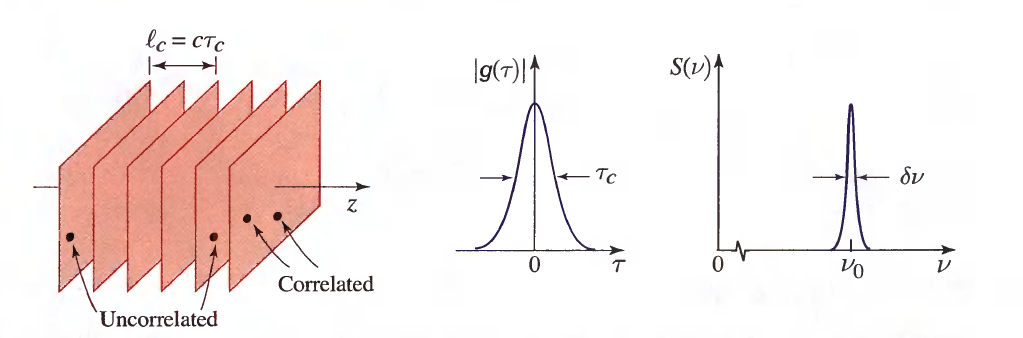
\includegraphics[width=0.9\textwidth]{11_1_9.PNG}
\caption{The fluctuations of a partially coherent plane wave at points on any wavefont (transverse plane) are completely correlated, whereas those at points on wavefronts separated by an axial distance greater than the coherence length $ l_c = c \tau_c $ are approximately uncorrelated.}
\label{fig: 11_1_9}
\end{figure}
\par In summary: the partially coherent plane wave is spatially coherent within each transverse plane, but partially coherent in the axial direction. The axial (longitudinal) spatial coherence of the wave has a one-to-one correspondence with the temporal coherence. The ratio of the coherence length $ l_c = c\tau_c $ to the maximun optical path difference $ l_{max} $ in the system governs the role played by coherence. If $ l_c \gg l_{max} $, the wave is effectively completely coherent. The coherence lengths of a number of light sources are listed in Table 11.1-2.
\bigbreak\noindent\textcolor{ksc}{\textbf{\textsl{Partially Coherent Spherical Wave}}}\\
A partially coherent spherical wave is described by the complex wavefunction (see Sec. 2.2B and Sec. 2.6A)
\begin{equation}
U(r, t) = \frac{1}{r} a(t - \frac{r}{c}) \exp[j\omega_0 (t - \frac{r}{c})],
\end{equation}
where $ a(t) $ is a random function. The corresponding mutual coherence function is 
\begin{equation}
G(r_1, r_2, \tau) = \frac{1}{r_1 r_2} G_a (\tau - \frac{r_2 - r_1}{c}) \exp [j\omega_0 (\tau - \frac{r_2 - r_1}{c})],
\end{equation}
with $ G_a (\tau) = \langle a^\ast (t) a(t+ \tau) \rangle $.
\par The intensity $ I(r) = G_a (0) / r^2 $ varies in accordance with an inverse-square law. The coherence time $ \tau_c $ is the width of the function $ \lvert g_a (\tau) \rvert = \lvert G_a (\tau) / G_a (0) \rvert $. It is the same everywhere in space. So is the power spectral density. For $ \tau =0 $, fluctuations at all points on a wavefront (a sphere) are completely correlated, wheras fluctuations at points on two wave fronts separated by the radial distance $ \lvert r_2 -r_1 \rvert \gg l_c = c\tau_c $ are uncorrelated (see Fig. 11.1-10).
\par An arbitrary partially coherent wave transmitted through a pinhole generates a partially coherent spherical wave. This process therefore imparts spatial coherence to the incoming wave (points on any sphere centered about the pinhole become completely correlated). However, the wave remains temporally partially coherent. Points at different distances from the pinhole are only partially correlated. The pinhole imparts spatial coherence but not temporal coherence to the wave.
\par Suppose now that an optial filter of very narrow spectral width is placed at the pinhole, so that the transmitted wave becomes approximately monochromatic. The wave will then have completely temporal, as well as spatial coherence. Temporal coherence is introduced by the narrowband filter, whereas spatial coherence is imparted by the pinhole, which acts as a spatial filter. The price for obtaining this idea wave is, of course, the loss of optical energy introduced by the temporal and spatial filtering process.
 \begin{figure}[H]
\centering
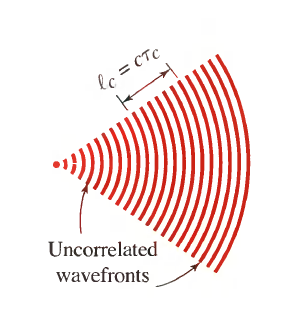
\includegraphics[width=0.3\textwidth]{11_1_10.PNG}
\caption{A partially coherent spherical wave has complete spatial coherence at all points on a wavefront, but not at points with different radial distances.}
\label{fig: 11_1_10}
\end{figure}

\bigbreak\begingroup
\color{ksc}
\subsection{INTERFERENCE OF PARTIALLY COHERENT LIGHT}
\endgroup
The interference of \textsl{coherent} light was discussed in Sec. 2.5. This section is devoted to the interference of partially \textsl{coherent} light.

\bigbreak\begingroup
\color{ksc}
\subsubsection{Interference of Two Partially Coherent Waves}
\endgroup
The statistical properties of two partially coherent waves $ U_1 $ and $ U_2 $ are described not only by their own mutual coherence functions but also by a measure of the degree to which their fluctuations are correlated. At a given position $ r $ and time $ t $, the intensities of the two waves are $ I_1 = \langle \lvert U_1 \rvert ^2 \rangle $ and $ I_2 = \langle \lvert U_2 \rvert ^2 \rangle $, whereas their cross-correlation is described by the statistical average $ G_{12} = \langle U_1^\ast U_2 \rangle $, and its normalized version
\begin{equation}
g_{12} = \frac{\langle U_1^\ast U_2 \rangle}{\sqrt{I_1 I_2}} .
\end{equation}
\par When the two waves are superposed, the average intensity of their sum is
\begin{align}
I = & \langle \lvert U_1 + U_2 \rvert ^2 \rangle = \langle \lvert U_1 \rvert ^2 \rangle + \langle \lvert U_2 \rvert ^2 \rangle + \langle U_1^\ast U_2 \rangle + \langle U_1 U_2^\ast \rangle \notag \\
={} & I_1 + I_2 + G_{12} + G_{12}^\ast = I1 + I2 + 2 Re\{ G_{12} \} \notag \\
={} & I_1 + I_2 + 2\sqrt{I_1 I_2}Re\{ g_{12} \},
\end{align}
from which
\begin{equation}
I = I_1 + I_2 + 2\sqrt{I_1 I_2} \lvert g_{12} \rvert \cos \varphi ,
\end{equation}
where $ \varphi = arg\{ g_{12} \} $ is the phase of $ g_{12} $. The third term on the right-hand side of (11.2-3) represents optical interference.
\par There are two important limits:
\bigbreak\par 1. For two completely correlated waves with $ g_{12} = \exp (j\varphi) $ and $ \lvert g_{12} \rvert = 1 $, we recover the interference formula (2.5-4) for two coherent waves of phase difference $ \varphi $.
\bigbreak\par 2. For two uncorrelated waves with $ g_{12} = 0 $, we have $ I = I_1 + I_2 $ so that there is no interference.
\bigbreak\par In the general case, the normalized intensity $ I $ versus the phase $ \varphi $ assumes the form of a sinusoidal pattern, as shown in Fig. 11.2-1. The strength of the interference is measured by \textbf{visibility} $ \mathcal{V} $ (also called the modulation depth or the contrast of the interference pattern):
\begin{equation}
\mathcal{V} = \frac{I_{max} - I_{min}}{I_{max} + I_{min}},
\end{equation}
where $ I_{max} $ and $ I_{min} $ are respectively, the maximum and minimum values that $ I $ takes as $ \varphi $ is varied. Since $ \cos \varphi $ stretches between 1 and -1, inserting (11.2-3) into (11.2-4) yields
\begin{equation}
\mathcal{V} = \frac{2\sqrt{I_1 I_2}}{I_1 + I_2} \lvert g_{12} \rvert .
\end{equation}
The visibility is therefore proportional to the absolute value of the normalized cross-correlation $ \lvert g_{12} \rvert $. In the special case when $ I_1 = I_2 $, we have
\begin{equation}
\mathcal{V} = \lvert g_{12} \rvert .
\end{equation}
 \begin{figure}[H]
\centering
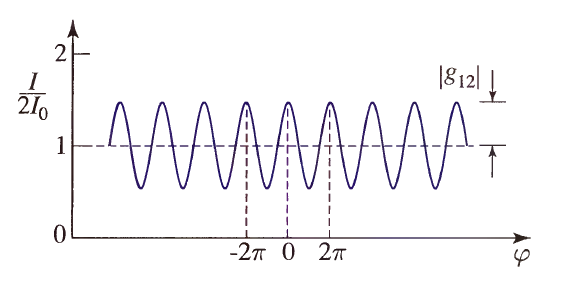
\includegraphics[width=0.3\textwidth]{11_2_1.PNG}
\caption{Normalized intensity $ I / 2I_0 $ of the sum of two partially coherent waves of equal intensities ($ I_1 = I_2 = I_0 $), as a function of the phase $ \varphi $ of their normalized cross-correlation $ g_{12} $. This sinusoidal pattern has visibility $ \mathcal{V} = \lvert g_{12} \rvert $.}
\label{fig: 11_2_1}
\end{figure}
\par The interference equation (11.2-3) will now be considered in a number of specific contexts to illustrate the effects that temporal and spatial coherence have on the interference of partially coherent light.
 
\bigbreak\begingroup
\color{ksc}
\subsubsection{Interference and Temporal Coherence}
\endgroup
Consider a partially coherent wave $ U(t) $ with intensity $ I_0 $ and complex degree of temporal coherence $ g(\tau) = \langle U^\ast (t) U(t + \tau) \rangle / I_0 $. If $ U(t) $ is added to a replica of itself delayed by the time $ \tau $, $ U(t + \tau) $, what is the intensity $ I $ of the superposition?
\par Using the interference formula (11.2-2) with $ U_1 = U(t) $, $ U_2 = U(t + \tau) $, $ I_1 = I_2 = I_0 $, and $ g_{12} = \langle U_1^\ast U_2 \rangle / I_0 = \langle U^\ast U(t + \tau) \rangle / I_0 = g(\tau) $, we obtain 
\begin{equation}
I = 2 I_0 [1 + Re\{g(\tau)\}] = 2 I_0 [1 + \lvert g(\tau) \rvert \cos \varphi (\tau)],
\end{equation}
where $ \varphi (\tau) = arg\{g(\tau)\}$. It is thus apparent that the ability of a wave to interfere with a time delayed replica of itself is governed by its complex degree of temporal coherence at that time delay.
\par Implementing the addition of a wave with a time-delayed replica of itself may be achieved by using a beamspliter to generate two identical waves, one of which is made to traverse a longer optical path than the other, and then recombining them at another (or the same) beamspliter. This can be effected, for example, with the help of a Mach-Zehnder or a Michelson interferometer (see Fig. 2.5-3).
\par Consider, as an example, the partially coherent plane wave introduced in Sec. 11.1D [see (11.1-31)], whose complex degree of temporal coherence is $ g(\tau) = g_a (\tau) \exp(j\omega_0 \tau) $. The spectral width of the wave is $ \Delta \nu_c = 1 / \tau_c $, where $ \tau_c $ (the width of $ \lvert g_a (\tau) \rvert $) is the coherence time. Substituting this into (11.2-7), we obtain
\begin{equation}
I = 2 I_0 \{1 + \lvert g_a (\tau) \rvert \cos [\omega_0 \tau + \varphi_a (\tau)]\} ,
\end{equation}
where $ \varphi_a (\tau) = arg \{g_a (\tau)\} $.
\par The relation between $ I $ and $ \tau $, which is known as an \textbf{interferogram}, is illustrated in Fig. 11.2-2. Assuming that $ \Delta \nu_c = 1 / \tau_c \ll \nu_0 $, the functions $ \lvert g_a (\tau) \rvert $ and $ \varphi_a (\tau) $ vary slowly in comparison with the period $ 1 / \nu_0 $. The visibility of this interferogram in the vicinity of a particular time delay $ \tau $ is $ \mathcal{V} = \lvert g(\tau) \rvert = \lvert g_a (\tau) \rvert $. It has a peak value of unity near $ \tau = 0 $ and vanishes for $ \tau \gg \tau_c $, i.e., when the optical path difference is much greater than the coherence length $ l_c = c\tau_c $. For the Michelson interferometer illustrated in Fig. 11.2-2, $\tau = 2(d_2 - d_1) / c $. Interference occurs only when the optical path differences is smaller than the coherence length.
 \begin{figure}[H]
\centering
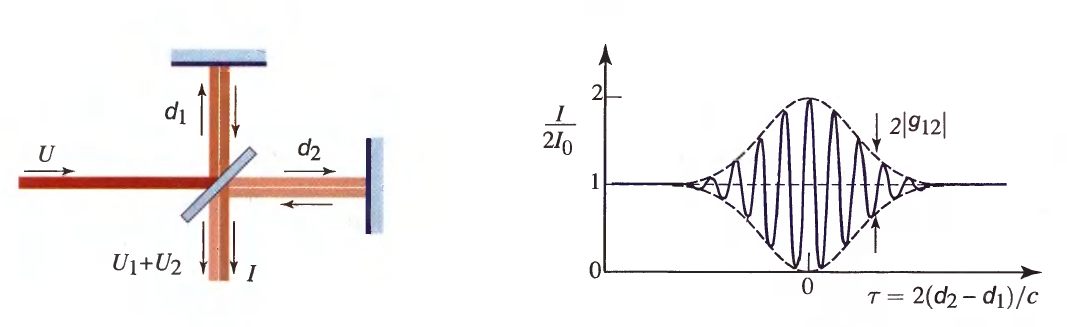
\includegraphics[width=0.9\textwidth]{11_2_2.PNG}
\caption{The normalized intensity $ I / 2I_0 $, as a function of time delay $ \tau $, when a partially coherent plane wave is introduced into a Michelson interferometer. The visibility determines the magnitude of the complex degree of temporal coherence.}
\label{fig: 11_2_2}
\end{figure}
\par The magnitude of the complex degree of temporal coherence of a wave, $\lvert g(\tau) \rvert $, may therefore be measured by monitoring the visibility of the interference pattern as a function of time delay. The phase of $ g(\tau) $ may be measured by observing the locations of the peaks of the pattern.
\bigbreak\noindent\textcolor{ksc}{\textbf{\textsl{Fourier-Transform Spectroscopy}}}\\
It is revealing to write (11.2-7) in terms of the power spectral density of the wave $ S(\nu) $. Using the Fourier-transform relation between $ G(\tau) $ and $ S(\nu) $,
\begin{equation}
G(\tau) = I_0 g(\tau) = \int_0^\infty S(\nu) \exp(j2\pi\nu\tau) \dif \nu ,
\end{equation}
substituting into (11.2-7), and noting that $ S(\nu) $ is real and that $ \int_0^\infty S(\nu) \dif \nu = I_0 $, we obtain
\begin{equation}
I = 2\int_0^\infty S(\nu) [1 + \cos(2\pi\nu\tau)] \dif \nu .
\end{equation}
This equation can be interpreted as a weighted superposition of interferograms produced by each of the monochromatic components of the wave. Each component $ \nu $ produces an interferogram with period $ 1 / \nu $ and unity visibility, but the composite interferogram exhibits reduced visibility by virtue of the different periods.
\par Equation (11.2-10) suggests that the spectral density $ S(\nu) $ of a light source can be determined by measuring the interferogram $ I $ versus $ \tau $ and then inverting the result by means of Fourier-transform methods. This technique is known as \textbf{Fourier-transform spectroscopy}.
\bigbreak\noindent\textcolor{ksc}{\textbf{\textsl{Optical Coherence Tomography}}}\\
\textbf{Optical coherence tomography} (OCT) is an interferometric technique for profiling a multilayered medium, i.e., for measuring the reflectance and depth of each of its boundaries. It makes use of a partially coherent light source of short coherence length and a Michelson interferometer. As illustrated in Fig. 11.2-3, a replica of the original wave, delayed by a moveable mirror, is superposed with a collection of waves reflected from the mutiple sample boundaries. Information about the sample profile is carried by the interferogram, which is the intensity measured at the detector as the movable mirror is translated. By virtue of the short coherence length of the source, the interferogram comprises sets of fringes centered at path delays of the movable mirror that match those of the reflecting boundaries.
 \begin{figure}[H]
\centering
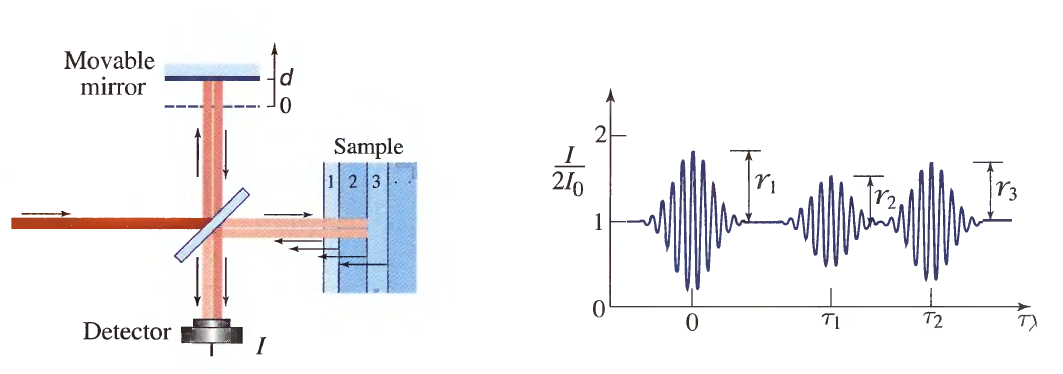
\includegraphics[width=0.9\textwidth]{11_2_3.PNG}
\caption{Optical coherence tomography.}
\label{fig: 11_2_3}
\end{figure}
\par Let $ U(t - \tau) $ be the wave reflected from the movable mirror, with its associated time delay $ \tau = d / c_0 $, and let $ r_i U(t - \tau_i), i = 1, 2, ..., $ be the waves reflected from the boundaries of the sample, where  $ r_i $ represents the amplitude reflectance at the $i$th boundary; the associated time delays are designated $ \tau_i $. For a symmetric beamspliter, the average intensity is the $ I(\tau) = \langle \lvert U(t - \tau) + \sum_i r_i U(t - \tau_i) \rvert ^2 \rangle $, which may be written in normalized form as 
\begin{equation}
I / 2I_0 = 1 + \sum_i r_i Re\{g(\tau - \tau_i)\} + \sum_{ij} r_i r_j^\ast Re\{g(\tau_j - \tau_i)\} ,
\end{equation}
since the complex degree of temporal coherence of the source is characterized by $ g(\tau) = \langle U^\ast (t) U(t + \tau)\rangle /$ $ \langle U^\ast (t) U(t) \rangle $.
\par The second term on the right-hand side of (11.2-11) is of paramount importance since it represents interference between the reference wave from the movable mirror and each of the waves reflected from the sample boundaries. The third term represents interference terms associated with mutiple reflections from the sample; since these terms are independent of the path delay of the movable mirror, $ \tau = d / c $, they may be regarded as background contributions and ignored.
\par For a light source of central frequency $ \nu_0 $, we have $ g(\tau) = g_a (\tau) \exp(j\omega_0 \tau) $, where the width of $ g_a (\tau) $ is the coherence time $ \tau_c $. Equation (11.2-11) then becomes
\begin{equation}
I / 2I_0 \approx 1 + \sum_i r_i \lvert g_a (\tau - \tau_i) \rvert \cos [\omega_0 (\tau - \tau_i) + \varphi_a (\tau - \tau_i)] ,
\end{equation}
where $ \varphi_a (r) = arg\{g_a ( \tau )\} $. If the source is of short coherence length, the function $ g_a (\tau) $ is narrow. As illustrated in Fig. 11.2-3, the reflection from each sample boundary then generates a distinct set of interference fringes of brief duration $ \tau_c $, centered about its corresponding time delay. Measurement of the OCT interferogram therefore permits the reflectance at each boundary, as well as the width of each of the sample layers, to be determined.
\par Optical coherence tomography has proven to be an effective imaging technique in clinical medicine as well as in engineering.

\bigbreak\begingroup
\color{ksc}
\subsubsection{Interference and Spatial Coherence}
\endgroup
The effect of spatial coherence on inerference is demonstrated by considering the Young's double-pinhole interference experiment, discussed in Exercise 2.5-2 for coherent light. A partially coherent optical wave $ U(r,t) $ illuminates an opaque screen with two pinholes loacted at positions $ r_1 $ and $ r_2 $. The wave has mutual coherence function $ G(r_1, r_2, \tau) = \langle U^\ast(r_1, t) U(r_2, t+\tau) \rangle $ and the complex degree of coherence $ g(r_1, r_2, \tau) $. The intensity is observed as a function of $x$. An important geometrical parameter is the angle $ \theta \approx 2a / d $ subtended by the two pinholes.
 \begin{figure}[H]
\centering
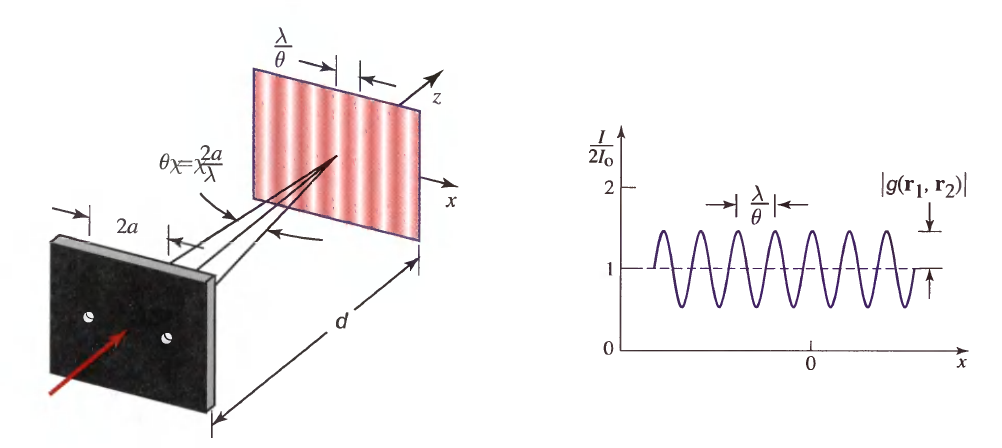
\includegraphics[width=0.9\textwidth]{11_2_4.PNG}
\caption{Young's double-pinhole interferometer. The incident wave is quasi-monochromatic and the normalized mutual intensity and the normalized mutual intensity at the pinholes is $ g(r_1, r_2) $. The normalized intensity $ I / 2 I_0 $ in the observation plane at a large distance is a sinusoidal function of $x$ with period $\lambda / \theta $ and visibility $ \mathcal{V} = \lvert g(r_1, r_2) \rvert $.}
\label{fig: 11_2_4}
\end{figure}
\par In the paraboloidal (Fresnel) approximation [see (2.2-17)], the two diffracted spherical waves are approximately related to $ U(r, t) $ by
\begin{subequations}
\begin{align}
U_1 (r, t) \propto U(r_1, t - \frac{\lvert r- r_1 \rvert}{c})  &\approx U(r_1, t - \frac{d + (x+a)^2 / 2d}{c})\\
U_2 (r, t) \propto U(r_2, t - \frac{\lvert r- r_2 \rvert}{c})  &\approx U(r_2, t - \frac{d + (x- a)^2 / 2d}{c}),
\end{align}
\end{subequations} 
and have approximately equal intensities, $ I_1 = I_2 = I_0 $. The normalized cross-correlation between the two waves at $r$ is
\begin{equation}
g_{12} = \frac{\langle U_1^\ast (r, t) U_2 (r, t) \rangle}{I_0} = g(r_1, r_2, \tau_x),
\end{equation}
where
\begin{equation}
\tau_x = \frac{\lvert r - r_1 \rvert - \lvert r - r_2 \rvert}{c} = \frac{(x + a)^2 - (x - a)^2}{2dc} = \frac{2ax}{dc} = \frac{\theta}{c}x
\end{equation}
is the difference in the time delays encountered by the two waves.
\par Substituting (11.2-14) into the interference formula (11.2-3) gives rise to an observed intensity $ I \equiv I(x) $:
\begin{equation}
I(x) = 2 I_0 [1 + \lvert g(r_1, r_2, \tau_x) \rvert \cos \varphi_x] ,
\end{equation}
where $ \varphi_x = arg\{g(r_1, r_2, \tau_x)\}$. This equation describes the pattern of observed intensity as a function of position $x$ in the observation plane, in terms of the magnitude and phase of the complex degree of coherence at the pinholes at time delay $ \tau_x = \theta_x / c$.
\bigbreak\noindent\textcolor{ksc}{\textbf{\textsl{Quasi-Monochromatic Light}}}\\
If the light is quasi-monochromatic with central frequency $ \nu_0 = \omega_0 / 2\pi$, i.e., if $ g(r_1, r_2, \tau_x) \approx g(r_1, r_2) \exp (j\omega_0 \tau_x) $, then (11.2-16) gives
\begin{equation}
I(x) = 2 I_0 [1 + \mathcal{V} \cos (\frac{2\pi \theta}{\lambda}x + \varphi)] ,
\end{equation}
where $ \lambda = c / \nu_0, \mathcal{V} = \lvert g(r_1, r_2) \rvert, \tau_x = \theta x / c $, and $ \varphi = arg\{g(r_1, r_2)\}$. The interference fringe pattern is therefore sinusoidal with spatial period $ \lambda / \theta $ and visibility $ \mathcal{V} $. In analogy with the temporal case, the visibility of the interference pattern equals the magnitude of the complex degree of spatial coherence at the two pinholes (Fig. 11.2-4). The locations of the peaks depend on phase $\varphi$.
\bigbreak\noindent\textcolor{ksc}{\textbf{\textsl{Interference with Light from an Extended Source}}}\\
If the incident wave in Young's interferometer is a coherent plane wave traveling in the $z$ direction, $ U(r,t) = \exp(-jkz) \exp(j\omega_0 t) $, then $ g(r_1, r_2) = 1 $, so that $ \lvert g(r_1, r_2) \rvert = 1 $, and $ arg\{g(r_1, r_2) = 0\} $. The interference pattern therefore has unity visibility and a peak at $ x = 0 $. But if the illumination is, instead, a tilted plane wave arriving from a direction in the $x-z$ plane making a small angle $\theta_x$ with respect to the z axis, i.e., $ U(r,t) \approx \exp[-j(kz + k\theta_x x)] \exp (j\omega_0 t) $, then $ g(r_1, r_2) = \exp(-jk\theta_x 2a) $.
The visibility remains $\mathcal{V} = 1 $, but the tilt results in a phase shift $ \varphi = -k\theta_x 2a = -2\pi \theta_x 2a / \lambda $, so that the interference pattern is shifted laterally by a fraction $ 2a \theta_x / \lambda $ of a period. When $ \varphi = 2\pi $, the pattern is shifted one period.
\par Suppose now that the incident light is a collection of independent plane waves arriving from a source that subtends an angle $ \theta_s $ at the pinhole plane(Fig. 11.2-5).
The phase shift $ \varphi $ then takes in the range $ \pm 2\pi (\theta_s / 2) 2a \lambda = \pm 2\pi \theta_s a / \lambda $ and the fringe pattern is a superposition of displaced sinusoids. If $ \theta_s = \lambda / 2a $, then $\varphi$ takes on values in the range $ \pm \pi $, which is sufficient to wash out the interference pattern and reduce its visibility to zero.
\begin{figure}[H]
\centering
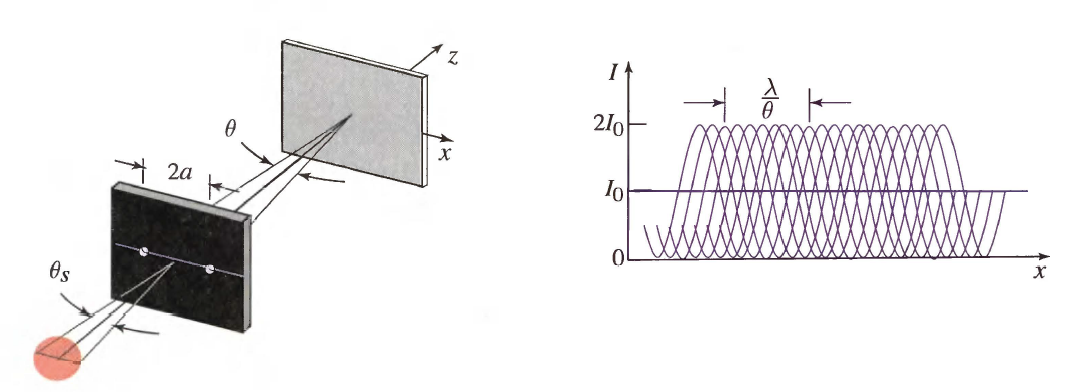
\includegraphics[width=0.9\textwidth]{11_2_5.PNG}
\caption{Young's interference fringes are washed out if the illumination emanates from a source of angular diameter $ \theta_s > \lambda / 2a $. If the distance $2a$ is smaller than $ \lambda / \theta_s $, the fringes become visible.}
\label{fig: 11_2_5}
\end{figure}
\par We conclude that the degree of spatial coherence at the two pinholes is very small when the angle subtended by the source is $ \theta_s = \lambda / 2a $ (or greater). Consequently, the distance
\begin{equation}
\rho_c \approx \frac{\lambda}{\theta_s}
\end{equation}
is a measure of the coherence distance in the plane of the screen and
\begin{equation}
A_c \approx (\frac{\lambda}{\theta_s})^2
\end{equation}
is a measure of the coherence area of light emitted from a source subtending an angle $\theta_s$. The angle subtended by the sun, for example, is $0.5 \degree$, so that the coherence distance for filtered sunlight of wavelength $\lambda$ is $\rho_c \approx \lambda / \theta_s \approx 115\lambda$. At $\lambda = 0.5 \mu m, \rho_c \approx 57.5 \mu m$.
A more rigorous analysis (see Sec. 11.3C)  shows that the transverse coherence distance $\rho_c$ for a circular incoherent light source of uniform intensity is 
\begin{equation}
\rho_c = 1.22 \frac{\lambda}{\theta_s} .
\end{equation}
\bigbreak\noindent\textcolor{ksc}{\textbf{\textsl{Effect of Spectral Width on Interference}}}\\
Finally, we examine the effect of the spectral width on interference in the Young's double-pinhole interferometer. The power spectral density of the incident wave is assumed to be a narrow function of width $\Delta \nu_c$ centered about $\nu_0$, and $\Delta \nu_c \ll \nu_0$. The complex degree of coherence then has the form
\begin{equation}
g(r_1, r_2, \tau) = g_a (r_1, r_2, \tau) \exp (j\omega_0 \tau),
\end{equation}
where $g_a (r_1, r_2, \tau)$ is slowly varying function of $\tau$ (in comparison with the period $1 / \nu_0$). Substituting (11.2-21) into (11.2-16), we obtain
\begin{equation}
I(x) = 2I_0 [1 + \mathcal{V}_x \cos(\frac{2\pi \theta}{\overline{\lambda}} + \varphi_x)] ,
\end{equation}
where $\mathcal{V}_x = \lvert g_a (r_1, r_2, \tau_x) \rvert , \varphi_x = arg\{g_a (r_1, r_2, \tau_x)\} , \tau_x = \theta x / c$, and $\overline{\lambda} = c / \nu_0$.
\par Thus, the interference pattern is sinusoidal with period $\overline{\lambda} / \theta$ but with a varying visibility $\mathcal{V}_x$ and varying phase $\varphi_x$ equal to the magnitude and phase of the complex degree of coherence at the two pinholes, respectively, evaluated at the time delay $\tau_x = \theta x / c$. If $\lvert g_a(r_1, r_2, \tau) \rvert= 1$ at $\tau = 0$, decreases with increasing $\tau$, and vanishes for $\tau \gg \tau_c$, the visibility $\mathcal{V}_x = 1$ at $x =0$, decreases with increasing $x$, and vanishes for $x \gg x_c = c\tau_c / \theta$. The interference pattern is then visible over a distance
\begin{equation}
x_c = \frac{l_c}{\theta} , 
\end{equation}
where $l_c = c\tau_c$ is the coherence length and $\theta$ is the angle subtended by the two pinholes (Fig. 11.2-6).
\begin{figure}[H]
\centering
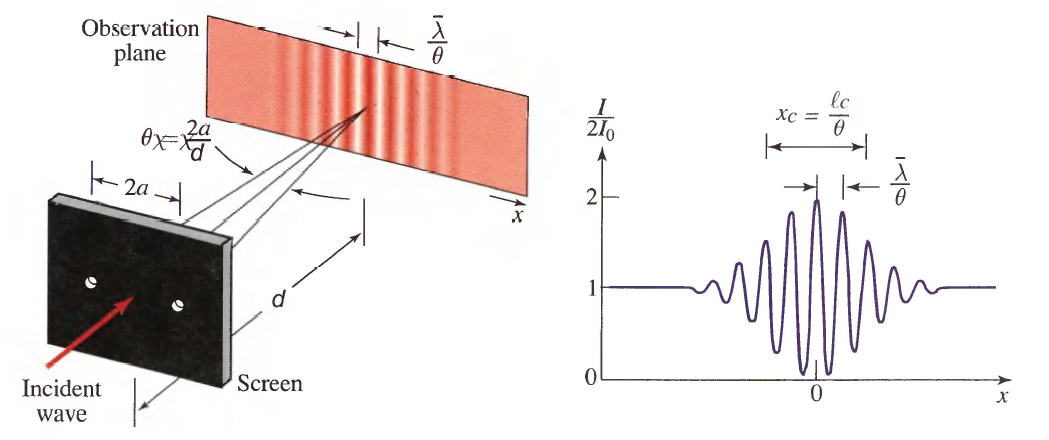
\includegraphics[width=0.9\textwidth]{11_2_6.PNG}
\caption{The visibility of Young's interference fringes at position $x$ is the magnitude of the complex degree of coherence at the pinholes at a time delay $\tau_x = \theta x / c$. For spatially coherent light,  the number of observable fringes is the ratio of the coherence length to the central wavelength, or the ratio of the central frequency to the spectral linewidth.}
\label{fig: 11_2_6}
\end{figure}
\par The number of observable fringes is thus $x_c / (\overline{\lambda} / \theta) = l_c / \overline{\lambda} = c\tau_c / \overline{\lambda} = \nu_0 / \Delta \nu_c$. It equals the ratio $l_c / \overline{\lambda}$ of the coherence length to the central wavelength, or the ratio $\nu_0 / \Delta \nu_c$ of the central frequency to the linewidth. Clearly, if $\lvert g(r_1, r_2, 0) \rvert < 1$, i.e., if the source is not spatially coherent, the visibility will be further reduced and even fewer fringes will be observable.

\bigbreak\begingroup
\color{ksc}
\subsection{TRANSMISSION OF PARTIALLY COHERENT LIGHT THROUGH OPTICAL SYSTEM}
\endgroup
The transmission of coherent light through thin optical components, through apertures, and through free space was discussed in Chapter 2 and 4. In this section we pursue the same goal for quasi-monochromatic partially coherent light. We assume that the spectral width is sufficently small so that the coherence length $l_c = c\tau_c = c / \Delta \nu_c$ is much greater than the differences of optical path lengths in the system. The mutual coherence function may then be approximated by $G(r_1, r_2, \tau) \approx G(r_1, r_2) \exp(j\omega_0 \tau)$, where $G(r_1, r_2)$ is the mutual intensity and $\nu_0$ is the central frequency.
\par It is noted at the outset that the transmission laws that apply to the deterministic function $U(r)$, which represents coherent light, apply also to the random function $U(r)$, which represents partially coherent light. However, for partially coherent light our interest is in the laws that govern statistical averages: the intensity $I(r)$ and the mutual intensity $G(r_1, r_2)$.

\bigbreak\begingroup
\color{ksc}
\subsubsection{Propagation of Partially Coherent Light}
\endgroup
\bigbreak\noindent\textcolor{ksc}{\textbf{\textsl{Transmission Through Thin Optical Componets}}}\\
When a partially coherent wave is transmitted through a thin optical component characterized by an amplitude transmittance $t(x,y)$,  the incident and transmitted waves are related by $U_2 (t) = t(r) U_1 (r)$, where $r = (x,y)$ is the position in the plane of the component (see Fig. 11.3-1). Using the definition of the mutual intensity, $G(r_1, r_2) = \langle U^\ast (r_1) U(r_2) \rangle$, we obtain
\begin{equation}
G_2 (r_1, r_2) = t^\ast (r_1) t(r_2) G_1(r_1, r_2) ,
\end{equation}
where $G_1(r_1, r_2)$ and $G_2(r_1, r_2)$ are the mutual intensities of the incident and transmitted light, respectively.
\begin{figure}[H]
\centering
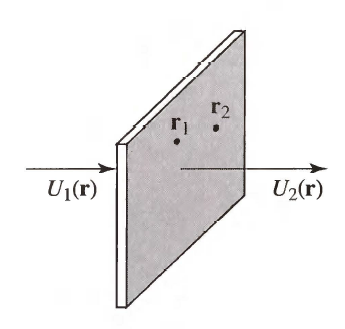
\includegraphics[width=0.3\textwidth]{11_3_1.PNG}
\caption{The absolute value of the degree of spatial coherence is not altered by transmission through a thin optical component.}
\label{fig: 11_3_1}
\end{figure}
\par Since the intensity at position $r$ equals the mutual intensity at $r_1 =  r_2 = r $,
\begin{equation}
I_2 (r) = \lvert t(r) \rvert ^2 I_1 (r) .
\end{equation}
The normalized mutual intensities defined by (11.1-27) therefore satisfy
\begin{equation}
\lvert g_2 (r_1, r_2) \rvert = \lvert g_1 (r_1, r_2) \rvert .
\end{equation}
Although transmission through a thin optical component may change the intensity of partially coherent light, it does not alter the magnitude of its degree of spatial coherence. Naturally, if the complex amplitude transmittance of the component itself were random, the coherence of the transmitted light would be altered.
\bigbreak\noindent\textcolor{ksc}{\textbf{\textsl{Transmission Through an Arbitrary Optical System}}}\\
We next consider an arbitrary optical system --- one that includes propagation in free space or transmission through thick optical components. It was shown in Chapter 4 that the complex amplitude $U_2 (r)$ at a point $r = (x,y)$ in the output plane of such a system is generally a weighted superposition integral comprising contributions from the complex amplitudes $U_1 (r')$ at points $r' = (x', y')$ in the input plane (see Fig. 11.3-2),
\begin{equation}
U_2 (r) = \int h(r; r') U_1 (r') \dif r' ,
\end{equation}
where $h(r, r')$ is the impulse response function of the system. The integral in (11.3-4) is a double integral with respect to $r' = (x', y')$ extending over the entire input plane.
\begin{figure}[H]
\centering
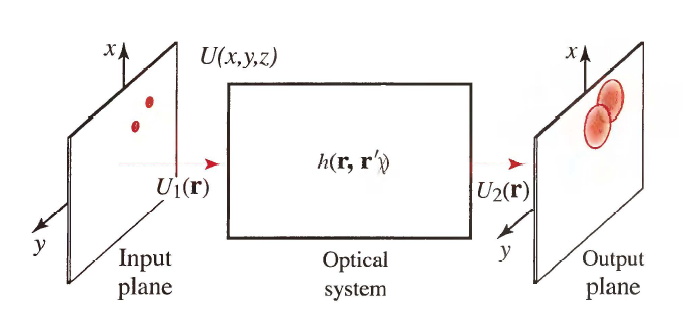
\includegraphics[width=0.7\textwidth]{11_3_2.PNG}
\caption{An optical system is characterized by its impulse response function $h(r; r')$.}
\label{fig: 11_3_2}
\end{figure}
\par To translate this relation between the random functions $U_2 (r)$ and  $U_1 (r')$ into a relation between their mutual intensities, we substitude (11.3-4) into the definition $G_2 (r_1, r_2) = \langle U_2^\ast (r_1) U_2(r_2) \rangle$
and use the definition $G_1(r'_1, r'_2) = \langle U_1^\ast (r'_1) U_1(r'_2) \rangle$ to obtain
\begin{equation}
G_2 (r_1, r_2) = \iint h^\ast (r_1; r'_1) h(r_2; r'_2) G_1 (r'_1, r'_2) \dif r'_1 \dif r'_2 .
\end{equation}
\par The intensity of the output light is obtained by using the definition $I_2 (r) = G_2 (r, r)$, which reduces (11.3-5) to
\begin{equation}
I_2 (r) = \iint h^\ast (r; r'_1) h(r; r'_2) G_1 (r'_1, r'_2) \dif r'_1 \dif r'_2 .
\end{equation}
To determine the intensity of the output light, we must know the mutual intensity of the input light. Knowledge of the input intensity $I_1 (r')$ by itself is generally not sufficient to determine the output intensity $I_2 (r)$.

\bigbreak\begingroup
\color{ksc}
\subsubsection{Image Formation with Incoherent Light}
\endgroup
We now consider the special case when the input light is incoherent. The mutual intensity $G_1 (r'_1, r'_2)$ vanishes when $r'_2$ is only slightly separated from $r'_1$ so that the coherence distance is much samller than other pertinent dimensions in the system (for example, the resolution distance of an imaging system). The mutual intensity may then be written in the form $G_1 (r'_1, r'_2) = \sqrt{I_1 (r'_1) I_1(r'_2)} g(r'_1 - r'_2)$, where $g(r'_1 - r'_2)$ is a very narrow function. When $G_1 (r'_1, r'_2)$ appears under the integral in (11.3-5) or (11.3-6),  it is convenient to replace $g(r'_1 - r'_2)$ with a delta function, $g(r'_1 - r'_2) = \sigma \delta (r'_1 - r'_2)$, where $\sigma = \int g(r') \dif r'$ is the area under $g(r')$, so that
\begin{equation}
G_1 (r'_1, r'_2) \approx \sigma \sqrt{I_1 (r'_1) I_1 (r'_2)} \delta (r'_1 - r'_2) .
\end{equation}
Since the mutual intensity must remain finite and $\delta (0) \to \infty$, this equation is clearly not generally accurate. It is valid only for the purpose of evaluating integrals such as in (11.3-6). Substituting (11.3-7) into (11.3-6), the delta function reduces the double integral and we obtain 
\begin{equation}
I_2 (r) = \int I_1 (r') h_i (r; r') \dif r' ,
\end{equation}
where
\begin{equation}
h_i (r; r') = \sigma \lvert h(r; r') \rvert ^2 .
\end{equation}
\par Under these conditions, the relation between the intensities at the input and ouput planes describes a linear system of impulse response function $h_i (r; r')$, also called the \textbf{point-spread function}. When the input light is completely incoherent, therefore, the intensity of the light at each point $r$ in the output plane is a weighted superposition of contributions from intensities at many points $r'$ of the input plane; interference does not occur and the intensities simply add (Fig. 11.3-3). This is to be contrasted with the completely coherent system, for which the complex amplitudes rather than intensities are related by a superposition integral, as in (11.3-4).
\begin{figure}[H]
\centering
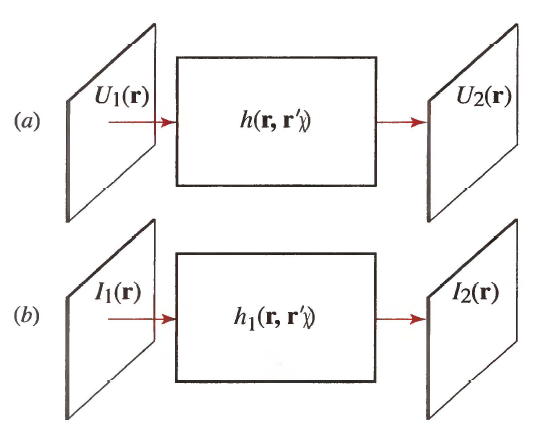
\includegraphics[width=0.5\textwidth]{11_3_3.PNG}
\caption{(a) The complex amplitudes of light at the input and output planes of an optical system illuminated by coherent light are related by a linear system with impulse response function $h(r; r')$. (b) The intensity of light at the input and output planes of an optical system illuminated by incoherent light are related by a linear system with impulse response function $h_i (r; r') = \sigma \lvert h(r; r') \rvert ^2$. }
\label{fig: 11_3_3}
\end{figure}
\par In certain optical systems the impulse response function is a function of $r-r'$, say $h(r - r')$. The system is then said to be shift variant or isoplanatic (see Appendix B). In this case $h_i (r; r') = h_i (r - r')$. The integrals in (11.3-4) and (11.3-8) are then two-dimensional convolutions and the systems can be described by transfer functions $H(\nu_x, \nu_y)$ and $H_i(\nu_x, \nu_y)$, which are the Fourier transforms of $h(r) = h(x,y)$ and  $h_i (r) = h_i (x,y)$, respectively.
\par As an example, we apply the relations above to an imaging system. It was shown in Sec. 4.4C that with coherent illumination, the impulse response function of the single-lens focused imaging system illustrated in Fig. 11.3-4 in the Fresnel approximation is
\begin{equation}
h(r) \propto P(\frac{x}{\lambda d_2}, \frac{y}{\lambda d_2}) ,
\end{equation}
where $P(\nu_x, \nu_y)$ is the Fourier transform of the pupil function $p(x, y)$ and $d_2$ is the distance from the lens to the image plane. The pupil function is unity within the aperture and zero elsewhere.
\begin{figure}[H]
\centering
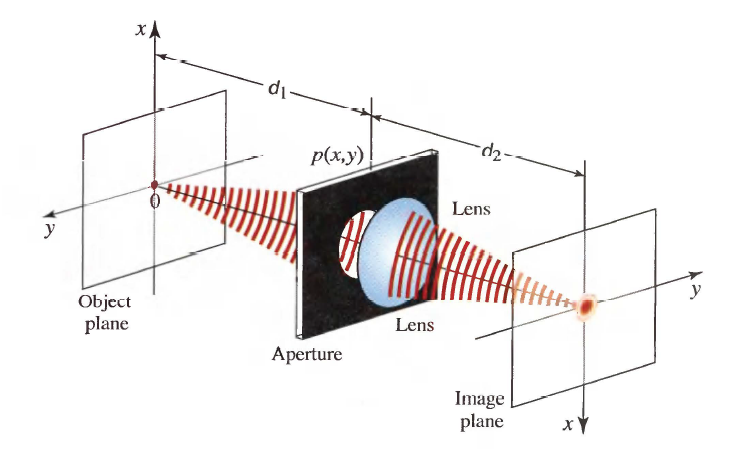
\includegraphics[width=0.7\textwidth]{11_3_4.PNG}
\caption{A single-lens imaging system.}
\label{fig: 11_3_4}
\end{figure}
\par When the illumination is quasi-monochromatic and spatially incoherent, the intensity of light at the object plane and image plane are linearly related by a system with impulse response function
\begin{equation}
h_i (r) = \sigma \lvert h(r) \rvert ^2 \propto \lvert P(\frac{x}{\lambda d_2}, \frac{y}{\lambda d_2}) \rvert ^2 ,
\end{equation}
where $\lambda$ is the wavelength corresponding to the central frequency $\nu_0$.\\
\noindent{\crule[ksc]{\textwidth}{0.1cm}}
\textbf{EXAMPLE 11.3-1. Imaging System with a Circular Aperture.} If the aperture is a circle of radius $a$, the pupil function $p(x,y) = 1$ for $x,y$ inside the circle, and 0 elsewhere. Its Fourier transform is
\begin{equation}
P(\nu_x, \nu_y) = \frac{a J_1 (2\pi \nu_\rho a)}{\nu_\rho} , \quad \nu_\rho = \sqrt{\nu_x^2 + \nu_y^2} ,
\end{equation}
where $J(\cdot)$ is the Bessel function (see Appendix A, Sec. A.3). This impulse response function of the coherent system is obtained by substituting into (11.1-36),
\begin{equation}
h(x,y) \propto [\frac{J_1 (2\pi\nu_s \rho)}{\pi\nu_s \rho}] , \quad \rho = \sqrt{x^2 + y^2} ,
\end{equation}
where 
\begin{equation}
\nu_s = \frac{\theta}{2 \lambda} , \quad \theta = \frac{2a}{d_2} .
\end{equation}
For incoherent illumination, the impulse response function is therefore
\begin{equation}
h_i (x,y) \propto [\frac{J_1 (2\pi\nu_s \rho)}{\pi\nu_s \rho}]^2 .
\end{equation}
\par The impulse response functions $h(x,y)$ and $h_i (x,y)$ are illustrated in Fig. 11.3-5. Both functions reach their first zero when $2\pi \nu_s \rho = 3.832$, or $\rho = \rho_s \approx 3.832 / 2\pi \nu_s = 3.832\lambda / \pi\theta$, from which
\begin{equation}
\rho_s \approx 1.22 \frac{\lambda}{\theta} .
\end{equation}
Thus the image of a point (impulse) in the input plane is a patch of intensity $h (x,y)$ or $h_i (x,y)$ and radius $\rho_s$. When the input distribution is composed of two points (impulses) separated by a distance $\rho_s$, the image of one point vanishes at the center of the image of the other point. The distance $\rho_s$ is therefore a measure of the resolution of the imaging system.
\begin{figure}[H]
\centering
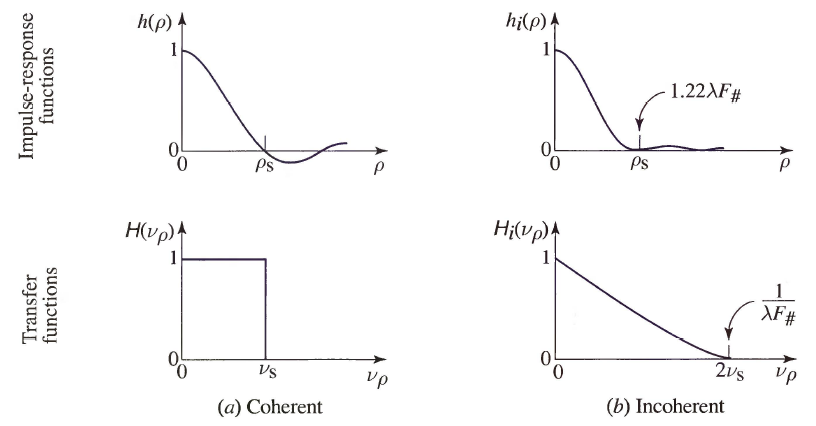
\includegraphics[width=0.9\textwidth]{11_3_5.PNG}
\caption{Impulse response functions and transfer functions of a single-lens focused diffraction-limited imaging system with a circular aperture and F-number $F_\#$ under (a) coherent and (b) incoherent illumination.}
\label{fig: 11_3_5}
\end{figure}
\par The transfer function of linear systems (see Appendix B) with impulse response functions $h(x,y)$ and $h_i (x,y)$ are the Fourier transforms (see Appendix A),
\begin{equation}
H(\nu_x, \nu_y) =
\begin{cases}
1, & \nu_\rho < \nu_s \\
0, & otherwise,
\end{cases}
\end{equation}
and
\begin{equation}
H_i (\nu_x, \nu_y) =
\begin{cases}
\frac{2}{\pi} \Big[\cos^{-1} \frac{\nu_\rho}{2\nu_s} -  \frac{\nu_\rho}{2\nu_s} \sqrt{1 - ( \frac{\nu_\rho}{2\nu_s})^2} \Big], & \nu_\rho < 2\nu_s \\
0, & otherwise,
\end{cases}
\end{equation}
where $\nu_\rho = \sqrt{v_x^2 + v_y^2}$. Both functions have been normalized such that their values at $\nu_\rho = 0$ are 1. These functions are illustrated in Fig. 11.3-5. For coherent illumination, the transfer function is flat and has a cutoff frequency $\nu_s = \theta / 2 \lambda$ lines/mm. For incoherent illumination, the transfer function drops approximately linearly with the spatial frequency and has a cutoff frequency $2\nu_s = \theta / \lambda$ lines/mm.
\par If the object is placed at infinity, i.e., $d_1 = \infty$, then $d_2 = f$, the focal length of the lens. The angle $\theta = 2a / f$ is then  the inverse of the lens F-number, $F_\# = f / 2a$. The cutoff frequencies $\nu_s$ and $2\nu_s$ are related to the lens F-number by
\begin{equation}
\text{Cutoff frequency(lines/mm)} =
\begin{cases}
\frac{1}{2 \lambda F_\#} & (\text{coherent illumination}) \\
\frac{1}{\lambda F_\#} & (\text{incoherent illumination}) .
\end{cases}
\end{equation}
\par One should not draw the false conclusion that incoherent illumination is superior to coherent illumination since it has twice the spatial bandwith. The transfer functions of the two systems should not be compared directly since one describes imaging of the complex amplitude, whereas the other describes imaging of the intensity.\\
\noindent{\crule[ksc]{\textwidth}{0.1cm}}

\bigbreak\begingroup
\color{ksc}
\subsubsection{Gain of Spatial Coherence by Propagation}
\endgroup
Equation (11.3-5) describes the change of the mutual intensity when light propagates through an optical system of impulse response function $h(r; r')$. When the input light is incoherent, the mutual intensity $G_1 (r'_1, r'_2)$ may be replaced by $\sigma \sqrt{I_1 (r'_1) I_1 (r'_2)} \delta (r'_1 - r'_2)$ and substituted in the double integral in (11.3-5) to obtain the single integral,
\begin{equation}
G_2 (r_1, r_2) = \sigma \int h^\ast (r_1; r) h(r_2; r) I_1 (r) \dif r .
\end{equation}
\par It is evident that the received light is no longer incoherent. In general, light gains spatial coherence by the mere act of propagation. This is not surprising. Although light fluctuations at different points of the input plane are uncorrelated, the radiation from each point spreads and overlaps with that from the neighboring points. The light reaching two points in the output plane comes from many points of the input plane, some of which are common (see Fig.11.3-6). These common contributions create partial correlation between fluctuations at the output points.
\par This is not unlike the transmission of an uncorrelated time signal (white noise) through a low-pass filter. The filter smooths the function and reduces its spectral bandwidth, so that its coherence time increases and it is no longer uncorrelated. The propagation of light through an optical system is a form of spatial filtering that cuts the spatial bandwidth and therefore increases the coherence area.
\begin{figure}[H]
\centering
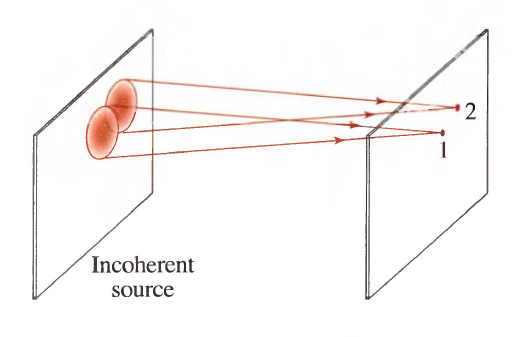
\includegraphics[width=0.5\textwidth]{11_3_6.PNG}
\caption{Gain of coherence by propagation is a result of the spreading of light. Although the light is completely uncorrelated at the source, the light fluctuations at points 1 and 2 share a common origin, the shaded area, and are therefore partially correlated.}
\label{fig: 11_3_6}
\end{figure}
\bigbreak\noindent\textcolor{ksc}{\textbf{\textsl{Van Cittert-Zernike Theorem}}}\\
There is a mathematical similarity between the gain of coherence of intially incoherent light propagating through an optical system, and the change of the amplitude of coherent light traveling through the same system. In reference to (11.3-20), if the observation point $r_1$ is fixed, for example at the origin 0, and the mutual intensity $G_2 (0, r_2)$ is examined as a function of $r_2$, then
\begin{equation}
G_2(0, r_2) = \sigma \int h^\ast (0; r) h(r_2; r) I_1 (r) \dif r .
\end{equation}
Defining $U_2 (r_2) = G_2 (0, r_2)$ and $U_1 (r) = \sigma h^\ast (0; r) I_1 (r)$, (11.3-21) may be written in the familiar  form
\begin{equation}
U_2(r_2) = \int h(r_2; r) U_1 (r) \dif r ,
\end{equation}
which is exactly the integral (11.3-4) that governs the propagation of coherent light. Thus, the observed mutual intensity $G(0, r_2)$ at the output of an optical system whose input is incoherent is mathematically identical to the observed complex amplitude if a coherent wave of complex amplitude $U_1 (r) = \sigma h^\ast (0; r) I_1 (r)$ were the input to the same system.
\par As an example, suppose that the incoherent input wave has uniform intensity and extends over an aperture $p(r)$ ($p(r) = 1$ within the aperture, and zero elsewhere),  i.e., $I_1 (r) = p(r)$; and assume that the optical system is free space; i.e., $h(r'; r) = \exp (-jk\lvert r' - r \rvert) / \lvert r' - r \rvert$. The mutual intensity $G_2 (0, r_2)$ is then identical to the amplitude $U_2 (r_2)$ obtained when a coherent wave with input amplitude $U_1 (r) = \sigma h^\ast (0; r) p(r) = \sigma p(r) \exp (jkr) / r$ is transmitted through the same system. This is a spherical wave converging to the point 0 in the output plane and transmitted through the aperture.
\par This similarity between the diffraction of coherent light and the gain of spatial coherence of incoherent light traveling through the same system is known as the \textbf{Van Cittert-Zernike theorem}.
\bigbreak\noindent\textcolor{ksc}{\textbf{\textsl{Gain of Coherence in Free Space}}}\\
Consider the optical system of free-space propagation between two parallel planes separated by a distance $d$ (Fig. 11.3-7). Light in the input plane is quasi-monochromatic, spatially incoherent, and has intensity $I(x,y)$ extending over a finite area. The distance $d$ is sufficiently large so that for points of interest in the output plane the Fraunhofer approximation is valid. Under these conditions the impulse response function of the optical system is described by the Fraunhofer diffraction formula [see (4.2-3)]
\begin{equation}
h(r; r') = h_0 \exp (-j\pi \frac{x^2 + y^2}{\lambda d}) \exp (j2\pi \frac{xx' + yy'}{\lambda d}),
\end{equation}
where $r = (x,y,d)$ and $r' = (x', y', 0)$ are the coordinates of points in the output and input planes, respectively, and $h_0 = (j / \lambda d) \exp(-j2\pi d / \lambda)$ is a constant.
\begin{figure}[H]
\centering
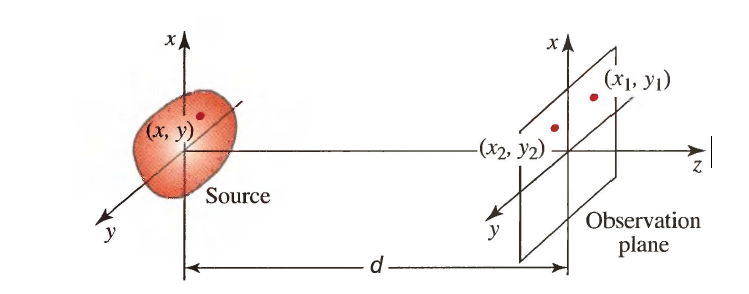
\includegraphics[width=0.8\textwidth]{11_3_7.PNG}
\caption{Radiation from an incoherent source in free space.}
\label{fig: 11_3_7}
\end{figure}
\par To determine the mutual intensity $G(x_1, y_1, x_2, y_2)$ at two points $(x_1, y_1)$ and $(x_2, y_2)$ in the output plane, we substitute (11.3-23) into (11.3-20) and obtain
\begin{equation}
\lvert G(x_1, y_1, x_2, y_2) \rvert = \sigma_1 \bigg\lvert \iint\limits_{-\infty}^{+\infty} \exp \{j\frac{2\pi}{\lambda d} [(x_2 - x_1)x + (y_2 - y_1)y]\}I(x,y) \dif x \dif y \bigg\rvert ,
\end{equation}
where $\sigma_1 = \sigma \lvert h_0 \rvert ^2 = \sigma / \lambda ^2 d^2$ is another constant. Given $I(x,y)$, one can easily determine $\lvert G(x_1, y_1, x_2, y_2) \rvert$ in terms of the two-dimensional Fourier transform of $I(x,y)$,
\begin{equation}
\mathcal{J} = \iint\limits_{-\infty}^{+\infty}\exp [j2\pi (\nu_x x+ \nu_y y)] I(x,y) \dif x \dif y
\end{equation}
evaluated at $\nu_x = (x_2 - x_1) / \lambda d$ and $\nu_y = (y_2 - y_1) / \lambda d$. The magnitude of the corresponding normalized mutual intensity is
\begin{equation}
\lvert g(x_1, y_1, x_2, y_2) \rvert = \bigg\lvert \mathcal{J}(\frac{x_2 - x_1}{\lambda d}, \frac{y_2 - y_1}{\lambda d}) \bigg\rvert / \mathcal{J}(0, 0) .
\end{equation}
This Fourier transform relation between the intensity profile of an incoherent source and the degree of spatial coherence of its far field is similar to the Fourier transform relation between the amplitude of coherent light and output  planes(see Sec. 4.2A). The similarity is expected in view of the Van Cittert-Zernike theorem.
\par The implications of (11.3-26) are profound. If the area of the source, i.e., the spatial extent of $I(x,y)$, is small, its Fourier transform $\mathcal{J}(\nu_x, \nu_y)$ is wide, so that the mutual intensity in the output plane extends over a wide area and the area of coherence in the output plane is large. In the extreme limit in which light in the input plane originates from a point, the area of coherence is infinite and the radiated field is spatially completely coherent. This confirms our earlier discussions in Sec. 11.1 D regarding the coherence of spherical waves. On the other hand, if the input spatially incoherent light originates from a large extended source, the propagated light has a small area of coherence.\\
\noindent{\crule[ksc]{\textwidth}{0.1cm}}
\textbf{EXAMPLE 11.3-2. Radiation from an Incoherent Circular Source.} For input light with uniform intensity $I(x,y) = I_0$ confined to a circular aperture of radius a, (11.3-26) yields
\begin{equation}
\lvert g(x_1, y_1, x_2, y_2) \rvert = \bigg\lvert \frac{2J_1(\pi\rho\theta_s / \lambda)}{\pi\rho\theta_s / \lambda} \bigg\rvert ,
\end{equation}
where $\rho = \sqrt{(x_2 - x_1)^2 + (y_2 - y_1)^2}$ is the distance between the two points, $\theta_s = 2a / d$ is the angle subtended by the source, and $J_1 (\cdot)$ is the Bessel function. This relation is plotted in Fig. 11.3-8. The Bessel function reaches its first zero when its argument is $3.832$. We can therefore define the area of coherence as a circle of radius $\rho_c = 3.832(\lambda / \pi\theta_s)$, so that
\begin{equation}
\rho_c = 1.22 \frac{\lambda}{\theta_s} .
\end{equation}
A similar result, (11.2-18), was obtained using a less rigorous analysis. The area of coherence is inversely proportional to $\theta_s^2$. An incoherent light source of wavelength $\lambda = 0.6 \mu$m and radius $1$cm
observed at a distance $d = 100$m, for example, has a coherence distance $\rho_c \approx 3.7$mm.
\begin{figure}[H]
\centering
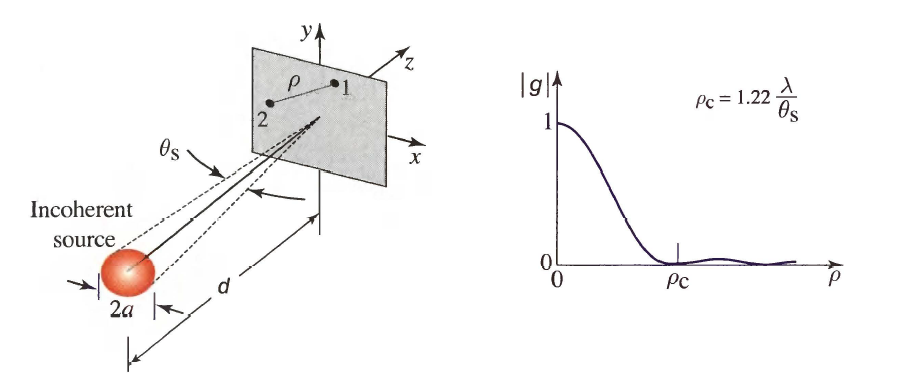
\includegraphics[width=0.8\textwidth]{11_3_8.PNG}
\caption{The magnitude of the degree of spatial coherence of light radiated from an incoherent circular light source subtending an angle $\theta_s$, as a function of the separation $\rho$.}
\label{fig: 11_3_8}
\end{figure}
\noindent{\crule[ksc]{\textwidth}{0.1cm}}
\bigbreak\noindent\textcolor{ksc}{\textbf{\textsl{Measurement of the Angular Diameter of Stars: The Michelson Stellar Interferometer}}}\\
Equation (11.3-28) is the basis of a method for measuring the angular diameters of stars. If the star is regarded as an incoherent disk of diameter $2a$ with uniform brilliance, then at an observation plane a distance $d$ away from the star, the mutual intensity drops to $0$ when the separation between the two observation points reaches $\rho_c = 1.22 \lambda / \theta_s$. Measuring $\rho_c$ for a given $\lambda$ permits us to determine the angular diameter $\theta_s = 2a / d$.
\par As an example, taking the angular diameter of the sun to be $0.5\degree$, $\theta_s = 8.7 \times 10^{-3}$ radians, and assuming that the intensity is uniform, we obtain $\rho_c = 140\lambda$. For $\lambda = 0.5 \mu$m, $\rho_c = 70 \mu$m. To observe interference fringes in a Young's double-slit apparatus, the slits would have to be separated by a distance smaller than 70 $\mu$m. Stars of smaller angular diameter have correspondingly larger areas of coherence. For example, the first star whose angular diameter was measured using this technique ($\alpha\text{-Orion}$) has an angular diameter $\theta_s = 22.6\times 10^{-8}$, so that for $\lambda = 0.57 \mu$m, $\rho_c = 3.1$m. A Young's interferometer can be modified to accommodate such large slit separations by using movable mirrors, as shown in Fig. 11.3-9.
\begin{figure}[H]
\centering
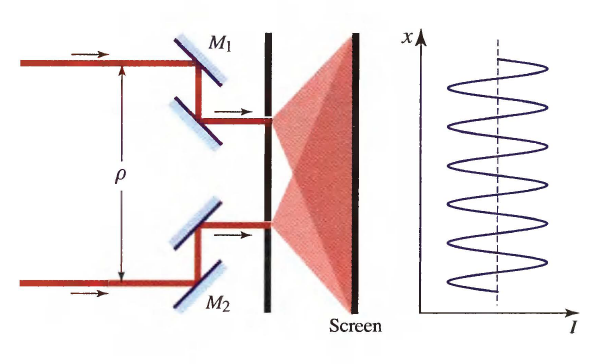
\includegraphics[width=0.5\textwidth]{11_3_9.PNG}
\caption{Michelson stellar interferometer. The angular diameter of a star is estimated by measuring the mutual intensity at two points with variable separation $\rho$ using Young's double-slit interferometer. The distance $\rho$ between mirrors $M_1$ and $M_2$ is varied and the visibility of the interference fringes is measured. When $\rho = \rho_c = 1.22\lambda / \theta_s$, the visibility = 0.}
\label{fig: 11_3_9}
\end{figure}

\bigbreak\begingroup
\color{ksc}
\subsection{PARTIAL POLARIZATION}
\endgroup
As we have seen in Chapter 6, the scalar theory of light is often inadequate and a vector theory that includes the polarization of light is necessary. This section provides a brief discussion of the statistical theory of random light, including the effects of polarization. The \textbf{theory of partial polarization} is based on characterizing the components of the optical field vector by correlations and cross-correlations similar to those defined earlier in this chapter.
\par To simplify the presentation, we shall not be concerned with spatial effects. We therefore limit ourselves to light described by a transverse electromagnetic (TEM) plane wave traveling in the z direction. The electric-field vector has two components in the $x$ and $y$ direction with complex wavefunctions $U_x (t)$ and $U_y (t)$ that are generally random. Each function is characterized by its autocorrelation function (the temporal coherence function),
\begin{align}
G_{xx}(\tau) &= \langle U_x^\ast (t) U_x(t + \tau) \rangle \\
G_{yy}(\tau) &= \langle U_y^\ast (t) U_y(t + \tau) \rangle .
\end{align}
An additional descriptor of the wave is the cross-correlation function of $U_x (t)$ and $U_y (t)$,
\begin{equation}
G_{xy}(\tau) = \langle U_x^\ast (t) U_y(t + \tau) \rangle .
\end{equation}
The normalized function
\begin{equation}
g_{xy} = \frac{G_{xy}(\tau)}{\sqrt{G_{xx}(0)G_{yy}(0)}}
\end{equation}
is the cross-correlation coefficient of $U_x (t)$ and $U_y(t + \tau)$. It satisfies the inequality $0 \le \vert g_{xy}(\tau) \rvert \le 1$. When the two components are uncorrelated at all times, $\lvert g_{xy}(\tau) \rvert = 0$; when they are completely correlated at all times, $\lvert g_{xy}(\tau) \rvert = 1$.
\par The spectral properties are, in general, tied to the polarization properties and the autocorrelation and cross-correlation functions can have different dependences on $\tau$. However, for quasi-monochromatic light, all dependences on $\tau$ in (11.4-1) to (11.4-4) are approximately of the form $\exp (j\omega_0 \tau)$, so that the polarization properties are described by the values at $\tau = 0$. The three numbers $G_{xx}(0), G_{yy}(0)$, and $G_{xy}(0)$, hereafter denoted $G_{xx}, G_{yy}$, and $G_{xy}$, are then used to describe the polarization of the wave. Note that $G_{xx} = I_x$ and $G_{yy} = I_y$ are real numbers that represent the intensities of the $x$ and $y$ components, but $G_{xy}$ is complex and $G_{yx} = G_{xy}^\ast$, as can easily be verified from the definition.
\bigbreak\noindent\textcolor{ksc}{\textbf{\textsl{Coherency Matrix}}}\\
It is convenient to write the four variables $G_{xx}, G_{xy}, G_{yx}$, and $G_{yy}$ in the form of a $2 \times 2$ Hermitian matrix
\begin{equation}
\mathbf{G} = 
\begin{bmatrix}
G_{xx} & G_{xy} \\
G_{yx} & G_{yy}
\end{bmatrix}
\end{equation}
called the \textbf{coherency matrix}. The diagonal elements are the intensities $I_x$ and $I_y$, and the off-diagonal elements are the cross-correlations. The trace of the matrix, $Tr\mathbf{G} = I_x + I_y  \equiv \bar{I}$, is the total intensity.
\par The coherency matrix may also be written in terms of the Jones vector, $\mathbf{J} = \begin{bmatrix}U_x \\ U_y \end{bmatrix}$, defined in terms of the complex wavefunctions and complex amplitudes (instead of in terms of the complex envelops as in Sec. 6.1B),
\begin{equation}
\langle \mathbf{J}^\ast \mathbf{J}^{\dag} \rangle = \langle 
\begin{bmatrix}
U_x^\ast \\
U_y^\ast
\end{bmatrix}
\begin{bmatrix}
U_x & U_y
\end{bmatrix}
\rangle =
\begin{bmatrix}
\langle U_x^\ast U_x \rangle & \langle U_x^\ast U_y \rangle \\
\langle U_y^\ast U_x \rangle & \langle U_y^\ast U_y \rangle 
\end{bmatrix}
= \mathbf{G} ,
\end{equation}
where $\dag$ denotes the transpose of a matrix, and $U_x$ and $U_y$ denote $U_x (t)$ and $U_y (t)$, respectively.
\par The Jones vector is transformed by polarization devices, such as polarizers and retarders, in accordance with the rule $\mathbf{J' = TJ}$ [see (6.1-17)], where $\mathbf{T}$ is the Jones matrix representing the device [see (6.1-18) to (6.1-25)]. The coherency matrix is therefore transformed in accordance with $\mathbf{ G' = \langle T^\ast J^\ast (TJ)^\dag \rangle = \langle T^\ast J^\ast J^\dag R^\dag \rangle} $ $\mathbf{= T^\ast \langle J^\ast J^\dag \rangle T^\dag}$, so that
\begin{equation}
\mathbf{G' = T^\ast G T^\dag} .
\end{equation}
We thus have a formalism for determining the effect of polarization devices on the coherency matrix of partially polarized light.
\bigbreak\noindent\textcolor{ksc}{\textbf{\textsl{Stokes Parameters and Poincar\'{e} Sphere Representation}}}\\
The Stokes parameters were defined in Sec. 6.1A for coherent light as a set of four real parameters related to the products of the x and y components of the complex envelope [see (6.1-9)]. This definition is readily generalized to partially coherent light as an average of these products:
\begin{subequations}
\begin{alignat}{3}
S_0 &= \langle \lvert U_x \rvert^2 \rangle + \langle \lvert U_y \rvert^2 \rangle &=& G_{xx} + G_{yy} \\
S_1 &= \langle \lvert U_x \rvert^2 \rangle - \langle \lvert U_y \rvert^2 \rangle &= &G_{xx} - G_{yy} \\
S_2 &= 2Re\{\langle U_x^\ast U_y \rangle \} &=& 2Re\{G_{xy} \} \\
S_3 &= 2Im\{\langle U_x^\ast U_y \rangle \} &= &2Im\{G_{xy} \} .
\end{alignat}
\end{subequations} 
Thus, the Stokes parameters are directly related to elements of the coherency matrix $\mathbf{G}$. The first parameter, $S_0$, is simply the sum of the diagonal elements, which is the total intensity $\bar{I}$. The second, $S_1$, is the difference of the diagonal elements, i.e., the difference between the intensities of the two polarization components. The third and fourth, $S_2$ and $S_3$, are proportional to the real and imaginary parts of the off-diagonal element, i.e., the cross-correlation function. Using these relations, it can be readily shown that the inequality $\lvert G_{xy} \rvert^2 \leq G_{xx}G_{yy}$ leads to the condition $S_1^2 + S_2^2 + S_3^2 \leq S_0^2$. Foe coherent light, these inequalities become equalities.
\par The state of polarization of partially polarized light may be represented geometrically on the Poincar\'{e} sphere as a point with Cartesian coordinates ($S_1 / S_0, S_2 / S_0, S_3 / S_0$). Since $S_1^2 + S_2^2 + S_3^2 \leq S_0^2$, such a point lies inside, or on, the surface of the sphere.
\par To understand the significance of the coherency matrix and the Stokes parameters, we next examine two limiting cases.
\bigbreak\noindent\textcolor{ksc}{\textbf{\textsl{Unpolarized Light}}}\\
Light of intensity $\bar{I}$ is said to be \textbf{unpolarized} if its two components have the same intensity and are uncorrelated, $I_x = I_y \equiv \frac{1}{2}\bar{I}$ and $G_{xy} = 0$. The coherency matrix is then
\begin{equation}
\mathbf{G} = \frac{1}{2}\bar{I}
\begin{bmatrix}
1 & 0 \\
0 & 1
\end{bmatrix}
\end{equation}
By use of (11.4-7) and (6.1-22), it can be shown that (11.4-9) is invariant to rotation of the coordinate system, so that two components always have equal intensities and are uncorrelated. Unpolarized light therefore has an electric field vector that is statistically isotropic; it is equally likely to have any direction in the $x-y$ plane, as illustrated in Fig. 11.4-1(a).
\begin{figure}[H]
\centering
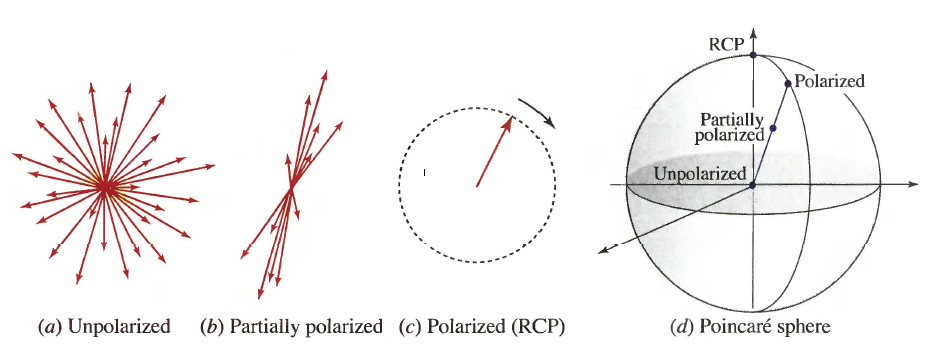
\includegraphics[width=0.9\textwidth]{11_4_1.PNG}
\caption{Fluctuations of electric field vector for (a) unpolarized light; (b) partially polarized light; (c) polarized light with circular polarization; (d) Poincar\'{e} representation.}
\label{fig: 11_4_1}
\end{figure}
\par When passed through a polarizer, unpolarized light becomes linearly polarized, but it remains random with an average intensity $\frac{1}{2}\bar{I}$. A wave retarder has no effect on unpolarized light since it only introduces a phase shift between two components that have a totally random phase to begin with. Similarly, unpolarized light transmitted through a polarization rotator remains unpolarized. These effects may be shown formally by use of (11.4-7) and (11.4.9) together with (6.1-18), (6.2-14), and (6.1-20).
\par Stokes parameters describing unpolarized light are $(S_0, S_1, S_2, S_3) = (\bar{I}, 0, 0, 0)$ as can be readily shown by use of (11.4-8) and (11.4-9). The corresponding representation on the Poincar\'{e} sphere is a point with Cartesian coordinates $(S_1 / S_0, S_2 / S_0, S_3 / S_0) = (0, 0, 0)$, i.e., is located at the very origin of the sphere.
\bigbreak\noindent\textcolor{ksc}{\textbf{\textsl{Polarized Light}}}\\
If the cross-correlation cofficient $g_{xy} = G_{xy} / \sqrt{I_x I_y}$ has unit magnitude, $\lvert g_{xy} \rvert = 1$, the two components of the optical field are perfectly correlated and the light is said to be completely polarized (or simply \textbf{polarized}). The coherency matrix then takes the form
\begin{equation}
\mathbf{G} = 
\begin{bmatrix}
I_x & \sqrt{I_x I_y}e^{j\varphi} \\
\sqrt{I_x I_y}e^{-j\varphi} & I_y
\end{bmatrix} ,
\end{equation}
where $\varphi$ is the argument of $g_{xy}$. Defining $U_x = \sqrt{I_x}$ and $U_y = \sqrt{I_y}e^{j\varphi}$,
\begin{equation}
\mathbf{G} =
\begin{bmatrix}
U_x^\ast U_x & U_x^\ast U_y \\
U_y^\ast U_x & U_y^\ast U_y
\end{bmatrix}
= \mathbf{J^\ast J^\dag} ,
\end{equation}
where $\mathbf{J}$ is a Jones vector with components $U_x$ and $U_y$. Thus, $\mathbf{G}$ has the same form as the coherency matrix of a coherent wave. Using the Jones vectors provided in Table 6.1-1, we can determine the coherency matrices for different states of polarization. Two examples are:
\begin{equation*}
\text{Linearly polarized in the $x$ direction} \quad \mathbf{G} = \bar{I}
\begin{bmatrix}
1 & 0 \\
0 & 0 
\end{bmatrix}
\quad \text{Right-circularly polarized} \quad \mathbf{G} = \frac{1}{2}\bar{I}
\begin{bmatrix}
1 & j \\
-j & 1
\end{bmatrix}
\end{equation*}
\par The Stokes parameters corresponding to (11.4-11) satisfy the relation $S_1^2 + S_2^2 + S_3^2 = S_0^2$, so that polarized light is represented by a point on the surface, rather than inside, the Poincar\'{e} sphere.
\par It is instructive to examine the distinction between unpolarized light and circularly polarized light. In both cases the intensities of the $x$ and $y$ components are equal $(I_x = I_y)$. For circularly polarized light the two components are completerly correlated, but for unpolarized light they are uncorrelated. Circularly polarized light may be transformed into linearly polarized light by the use of a wave retarder, but unpolarized light remains unpolarized upon passage through such a device. Circularly polarized light is represented by a point at the north or sourth poles of the Poincar\'{e} sphere, while unpolarized light is represented by a point at the origin.
\bigbreak\noindent\textcolor{ksc}{\textbf{\textsl{Degree of Polarization}}}\\
Partial polarization is a general state of random polarization that lies between the two ideal limits of unpolarized and polarized light. One measure of the \textbf{degree of polarization} is defined in terms if the determinant and the trace of the coherency matrix:
\begin{align}
\mathbb{P} &= \sqrt{1 - \frac{4 det \mathbf{G}}{(Tr \mathbf{G})^2}} \\
&= \sqrt{1-4\frac{I_x I_y}{(I_x + I_y)^2}(1 - \lvert g_{xy} \rvert^2)} .
\end{align}
This measure is meaningful because of the following considerations:
\par$\sqcdot$ It satisfies the inequality $0 \leq \mathbb{P} \leq 1$.
\par$\sqcdot$ For polarized light, $\mathbb{P}$ has its highest value of 1, as can easily be seen by substituting $\lvert g_{xy} = 1 \rvert$ into (11.4-13). For unpolarized light it has its lowest value $\mathbb{P} = 0$, since $I_x = I_y$ and $g_{xy} = 0$.
\par$\sqcdot$ It is invariant to rotation of the coordinate system (since the determinant and the trace of a matrix are invariant to unitary transformations).
\par$\sqcdot$ The degree of polarization in (11.4-13) may also be expressed in terms of the Stokes parameters as:
\begin{equation}
\mathbb{P} = \frac{\sqrt{S_1^2 + S_2^2 + S_3^2}}{S_0} ,
\end{equation}
\par$\phantom{\sqcdot}$ so that in the Poincar\'{e} sphere representation, it is equal to the distance from the origin of the sphere.
\par$\sqcdot$ It can be shown (Exercise 11.4-1) that a partially polarized wave can always be regarded as a mixture of two uncorrelated waves: a completely polarized wave and an unpolarized wave, with the ratio of the intensity component to the total intensity equal to the degree of polarization $\mathbb{P}$.\\
\noindent{\crule[ksc]{\textwidth}{0.2cm}}
\textbf{EXERCISE 11.4-1} \\
\textbf{Partially Polarized Light.} Show that the superposition of unpolarized light of intensity $(I_x + I_y)(1 - \mathbb{P})$, and linearly polarized light with intensity $(I_x + I_y)\mathbb{P}$, where $\mathbb{P}$ is given by (11.4-13), yields light whose $x$ and $y$ components have intensities $I_x$ and $I_y$ and normalized cross-correlation $\lvert g_{xy} \rvert$.\\
\noindent{\crule[ksc]{\textwidth}{0.2cm}}

\clearpage
\pagestyle{empty}
\bigbreak\textcolor{ksc}{\huge{\textbf{\centerline{READING LIST}}}}\\
\begin{spacing}{0.5}
\bigbreak\noindent{\large\textbf{\textsl{General}}}\\
\begin{hangparas}{0.25cm}{1}
\par A. A. Kokhanovsky, Polarization Optics of Random Media, Springer-Verlag, 2003.\\
\par E. L. O'Neill, Introduction to Statistical Optics, Addison-Wesley, 1963; Dover, reissued 2003.\\
\par W. Lauterborn and T. Kurz, Coherent Optics: Fundamentals and Applications, Springer, 2nd ed.
2003.\\
\par M. Born and E. Wolf, Principles of Optics, Cambridge University Press, 7th expanded and corrected
ed. 2002, Chapter 10.\\
\par B. R. Frieden, Probability, Statistical Optics, and Data Testing: A Problem Solving Approach,
Springer-Verlag, 1983, 3rd ed. 2001.\\
\par J. W. Goodman, Statistical Optics, Wiley, 1985, paperback ed. 2000.\\
\par H. E. Rowe, Electromagnetic Propagation in Multi-Mode Random Media, Wiley, 1999.\\
\par C. Brosseau, Fundamentals of Polarized Light: A Statistical Optics Approach, Wiley, 1998.\\
\par L. Mandel and E. Wolf, Optical Coherence and Quantum Optics, Cambridge University Press, 1995.\\
\par H. Le£ 七vre, The Fiber-Optic Gyroscope, Artech, 1993.\\
\par G. Reynolds, J.B. De Velis, G. B. Parrent, and B. J. Thompson, The New Physical Optics Notebook:
\par Tutorials in Fourier Optics, SPIE Optical Engineering Press, 1989.\\
\par J. Perina, Coherence of Light, Reidel, 1971, 2nd ed. 1985.\\
\par J.C. Dainty, ed., Laser Speckle and Related Phenomena, Springer-Verlag, 1975, 2nd ed. 1984.\\
\par A. S. Marathay, Elements of Optical Coherence Theory, Wiley, 1982.\\
\par B. E. A. Saleh, Photoelectron Statistics with Applications to Spectroscopy and Optical Communication, Springer-Verlag, 1978.\\
\par B. Crosignani, P. Di Porto, and M. Bertolotti, Statistical Properties of Scattered Light, Academic
Press, 197 5.\\
\par M. J. Beran and G. B. Parrent, Jr., Theory of Partial Coherence, Prentice Hall, 1964; SPIE Optical
Engineering Press, reissued 1974.\\
\par R. Hanbury-Brown, The Intensity Interferometer: Its Application to Astronomy, Taylor \& Francis,
1974.\\
\par G. J. Troup, Optical Coherence Theory', Methuen, 1967.\\


\bigbreak\noindent{\large\textbf{\textsl{Books on Random Functions}}}\\
\par A. Papoulis and S. U. Pillai, Probability, Random Variables, and Stochastic Processes, McGraw-Hill,
1965, 4th ed. 2002.\\
\par E. Parzen, Stochastic Processes, Holden-Day, 1962; Society for Industrial and Applied Mathematics
(SIAM), reissued 1999.\\
\par E. Parzen, Modern Probability Theory and Its Applications, Wiley, 1960, paperback ed. 1992.\\
\par C. W. Helstrom, Probability and Stochastic Processes for Engineers and Scientists, Macmillan, 2nd.
ed. 1991.\\
\par W. B. Davenport, Jr., and W. L. Root, An Introduction to the Theory of Random Signals and Noise,
McGraw-Hill, 1958; IEEE Press, reissued 1987.\\
\par E. Vanmarcke, Random Fields, MIT Press, 1983.\\
\par J.B. Thomas, An Introduction to Applied Probability and Random Processes, Wiley, 1971.\\


\bigbreak\noindent{\large\textbf{\textsl{Books on Optical Coherence Tomography}}}\\
\par M. E. Brezinski, Optical Coherence Tomography: Principles and Applications, Academic Press,
2006.\\
\par W. Drexler, ed., Optical Coherence Tomography and Coherence Techniques, Volume 2, Progress in Biomedical Optics and Imaging, SPIE Optical Engineering Press, 2005.\\
\par W. Drexler, ed., Optical Coherence Tomography and Coherence Techniques, Volume 1, Progress in
Biomedical Optics and Imaging, SPIE Optical Engineering Press, 2003.\\
\par B. E. Bouma and G. J. Teamey, eds., Handbook of Optical Coherence Tomography, Marcel Dekker,
2002.\\


\bigbreak\noindent{\large\textbf{\textsl{Articles}}}\\
\par P. H. Tomlins and R. K. Wang, Theory, Developments and Applications of Optical Coherence Tomography,
\par Journal of Physics D: Applied Physics, vol. 38, pp. 2519—2535, 2005.\\
\par A. F. Fercher, W. Drexler, C. K. Hitzenberger, and T. Lasser, Optical Coherence Tomography—
Principles and Applications, Reports on Progress in Physics, vol. 66, pp. 239-303, 2003.\\
\par L. Mandel and E. Wolf, eds., Selected Papers on Coherence and Fluctuations of Light (1850-1966), SPIE Optical Engineering Press (Milestone Series Volume 19), 1990.\\
\par R. B. Smith, ed., Selected Papers on Fiber Optic Gyroscopes, SPIE Optical Engineering Press (Milestone Series Volume 8), 1989.\\
\par Feature issues on applications of coherence and statistical optics, Journal of the Optical Society of
America, no. 7, 1986 and no. 8, 1986.\\
\par F. T. S. Yu, Principles of Optical Processing with Partially Coherent Light, in Progress in Optics,
vol. 23, E. Wolf, ed., North-Holland, 1986.\\
\par W. J. Tango and R. Q. Twiss, Michelson Stellar Interferometry, in Progress in Optics, vol. 17, E. Wolf,
ed., North-Holland, 1980.\\
\par G. 0. Reynolds and J.B. De Velis, Review of Optical Coherence Effects in Instrument Design, SPIE
Proceedings, vol. l94, pp. 2-33, 1979.\\
\par H. P. Baltes, J. Geist, and A. Walther, Radiometry and Coherence, in Inverse Source Problems in
Optics, H. P. Baltes, ed., Springer-Verlag, 1978.\\
\par E. Wolf, Coherence and Radiometry, Journal of the Optical Society of America, vol. 68, pp. 6-17,
1978.\\
\par L. Mandel and E. Wolf, eds., Selected Papers on Coherence and Fluctuations of Light, Volumes .l
and 2, Dover, 1970.\\
\par B. J. Thompson, Image Formation with Partially Coherent Light, in Progress in Optics, vol. 7,
E. Wolf, ed., North-Holland, 1969.\\
\par L. Mandel and E. Wolf, Coherence Properties of Optical Fields, Reviews of Modem Physics, vol. 37,
pp.231-287, 1965.\\
\end{hangparas}
\end{spacing}

\bigbreak\textcolor{ksc}{\huge{\textbf{\centerline{PROBLEMS}}}}
\bigbreak
{
\setlength{\parskip}{2ex}
\begin{hangparas}{1.4cm}{1}
\par 11.1-4 \quad\textbf{Lorentzian Spectrum.} A light-emitting diode (LED) emits light of Lorentzian spectrum with a linewidth $\Delta\nu (FWHM) = 10^{13} Hz$ centered about a frequency corresponding to a wavelength $\lambda_0 = 0.7 \mu m$. Determine the linewidth $\Delta\lambda_0$ (in units of nm), the coherence time $\tau_c$, and the coherence length $l_c$. What is the maximum time delay within which the magnitude of the complex degree of temporal coherence $\lvert g(\tau) \rvert$ is greater than 0.5?
\par 11.1-5 \quad\textbf{Proof of the Wiener-Khinchin Theorem.} Use the definitions in (11.1-4), (11.1-14), and (11.1-15) to prove that the spectral density $S(\nu)$ is the Fourier transform of the autocorrelation function $G(\tau)$. Prove that the intensity $I$ is the integral of the power spectral density $S(\nu)$.
\par 11.1-6 \quad\textbf{Mutual intensity.} The mutual intensity of an optical wave at points on the $x$ axis is given by
\begin{equation*}
G(x_1, x_2) = I_0 \exp [- \frac{(x_1^2 + x_2^2)}{W_0^2}]\exp [- \frac{(x_1 - x_2)^2}{\rho_c^2}] ,
\end{equation*}
where $I_0, W_0$, and $\rho_0$ are constants. Sketch the intensity distribution as a function a $x$. Derive an expression for the normalized mutual intensity $g(x_1, x_2)$ and sketch it as a function of $x_1 - x_2$. What is the physical meaning of the parameters $I_0, W_0$, and $\rho_c$?
\par 11.1-7 \quad\textbf{Mutual Coherence Function.} An optical wave has a mutual coherence function at points on the $x$ axis,
\begin{equation*}
G(x_1, x_2, \tau) = \exp (- \frac{\pi \tau^2}{2 \tau_c^2})\exp [j2\pi \mu (x_1, x_2)\tau] \exp[- \frac{(x_1 - x_2)^2}{\rho_c^2}] ,
\end{equation*}
where $u(x_1, x_2) = 5 \times 10^{14} s^{-1}$ for $x_1 + x_2 > 0$, and $6 \times 10^{14} s^{-1}$ for $x_1 + x_2 < 0$, $\rho_c = 1 mm$, and $\tau_c = 1\mu s$. Determine the intensity, the power spectral density, the coherence length, and the coherence distance in transverse plane. Which of these quantities is position independent? If this wave were recorded on color film, what would the recorded image look like?
\par 11.1-8 \quad\textbf{Coherence Length.} Show that light of narrow spectral width has a coherence length $l_c \approx \lambda^2 / \Delta\lambda$, where $\Delta\lambda$ is the linewidth in wavelength units. Show that for light of broad uniform spectrum extending between the wavelengths $\lambda_{min}$ and $\lambda_{max} = 2\lambda_{min}$, the coherence length $l_c = \lambda_{max}$.
\par 11.1-9 \quad\textbf{Effect of Spectral Width on Spatial Coherence.} A point source at the origin $(0, 0, 0)$ of a Cartesian coordinate system emits light with a Lorentzian spectrum and coherence time $\tau_c = 10 ps$. Determine an expression for the normalized mutual intensity of the light at the points $(0, 0, d)$ and $(x, 0, d)$, where $d = 10 cm$. Sketch the magnitude of the normalized mutual intensity as a function of $x$.
\par 11.1-10 \quad\textbf{Gaussian Mutual Intensity.} An optical wave in  free space has a mutual coherence function $G(r_1, r_2, \tau) = J(r_1 - r_2)\exp j\omega_0 \tau$.\\
(a) Show that the function $J(r)$ must satisfy the Helmholtz equation $\nabla^2 J + k_0^2 J = 0$, where $k_0 = \omega_0 / c$.\\
(b) An approximate solution of the Helmholtz equation is the Gaussian-beam solution
\begin{equation*}
J(r) = \frac{1}{q(z)}\exp [- \frac{jk_0 (x^2 + y^2)}{2q(z)}]\exp(- jk_0 z),
\end{equation*}
where $q(z) = z + jz_0$ and $z_0$ is a constant. This solution has been studied extensively in Chapter 3 in connection with Gaussian beams. Determine an expression for the coherence area near the $z$ axis and show that it increases with $\lvert z \rvert$, so that the wave gains coherence with propagation away from the origin.
\par 11.2-1 \quad\textbf{Effect of Spectral Width on Fringe Visibility.} Light from a sodium lamp of Lorentzian spectral linewidth $\Delta \nu = 5 \times 10^{11} Hz$ is used in a Michelson interferometer. Determine the maximum path-length difference for which the visibility of the interferogram $\mathcal{V} > \frac{1}{2}$.
\par 11.2-2 \quad\textbf{Number of Observable Fringes in Young's Interferometer.} Determine the number of observable fringes in Young's interferometer if each of the sources in Table 11.1-2 is used. Assume full spatial coherence in all cases.
\par 11.2-3 \quad\textbf{Spectrum of a Superposition of Two Waves.} An optical wave is a superposition of two wave $U_1(t)$ and $U_2(t)$ with identical spectra $S_1(\nu) = S_2(\nu)$, which are Gaussian with spectral width $\Delta\nu$ and central frequency $\nu_0$. The waves are not necessarily uncorrelated. Determine an expression for the power spectral density $S(\nu)$ of the superposition $U(t) = U_1(t) + U_2(t)$. Explore the possibility that $S(\nu)$ is also Gaussian, with a shift central frequency $\nu_1 \neq \nu_0$. If this were possible, our faith in using the Doppler shift as a method to determine the velocity of stars would be be shaken, since frequency shifts could originate from something other than the Dopper effect.
\par$\prescript{\ast}{}{11}$.3-1 \quad\textbf{Partially Coherent Gaussian Beam.} A quasi-monochromatic light wave of wavelength $\lambda$ travels in free space in the $z$ direction. Its intensity in the $z = 0$ plane is a Gaussian function $I(x) = I_0 \exp(- 2x^2 / W_0^2)$ and its normalized mutual intensity is also a Gaussian function $g(x_1, x_2) = \exp [-(x_1 - x_2)^2 / \rho_c^2]$. Show that the intensity at a distance $z$ satisfying conditions of the Fraunhofer approximation is also a Gaussian function $I_z (x) \propto \exp [- 2x^2 / W^2 (z)]$ and derive an expression for the beam width $W(z)$ as a function of $z$ and the parameters $W_0, \rho_c$, and $\lambda$. Discuss the effect of spatial coherence on beam divergence.
\par$\prescript{\ast}{}{11}$.3-2 \quad\textbf{Fourier-Transform Lens.} Quasi-monochromatic spatially incoherent light of uniform intensity illuminates a transparency of intensity transmittance $f(x, y)$ and the emergent light is transmitted between the front and back focal planes of a lens. Determine an expression for the intensity of the observed light. Compare your results with the case of the coherent light in which the lens performs the Fourier transform (see Sec. 4.2).
\par$\prescript{\ast}{}{11}$.3-3 \quad\textbf{Light from Two-Point Incoherent Source.} A spatially incoherent quasi-monochromatic source of light emits only at two points separated by a distance $2a$. Determine an expression for the normalized mutual intensity at a distance $d$ from the source (use the Fraunhofer approximation).
\par$\prescript{\ast}{}{11}$.3-4 \quad\textbf{Coherence of Light Transmitted Through a Fourier-Transform Optical System.} Light from a quasi-monochromatic spatially incoherent source with uniform intensity is transmitted through a thin slit of width $2a$ and travels between the front and back focal planes of a lens. Determine an expression for the normalized mutual intensity in the back focal plane.
\par 11.2-3 \quad\textbf{Partially Polarized Light.} The intensities of the two components of a partially polarized wave are $I_x = I_y = \frac{1}{2}$, and the argument of the cross-correlation coefficient $g_{xy}$ is $\pi / 2$.\\
(a) Plot the degree of polarization $\mathbb{P}$ versus the magnitude of the cross-correlation coefficient $\lvert g_{xy} \rvert$.\\
(b) Determine the coherency matrix if $\mathbb{P} = 0, 0.5$, and $1$, and describe the nature of the light in each case.\\
(c) If the light is transmitted through a polarizer with its axis in the $x$ direction, what is the intensity of the light transmitted?
\end{hangparas}
}
\end{document}
